\documentclass[a4paper,10pt]{book}
\usepackage[utf8x]{inputenc}
\usepackage[T1]{fontenc}
%\usepackage{ae,aecompl}
    
\usepackage{makeidx}         % allows index generation
\usepackage{graphicx}        % standard LaTeX graphics tool
                             % when including figure files
\usepackage{multicol}        % used for the two-column index
\usepackage[bottom]{footmisc}% places footnotes at page bottom

\makeindex             % used for the subject index
                       % please use the style sprmidx.sty with
                       % your makeindex program

%packages
\usepackage[all,arc,curve,color,frame]{xy}
\usepackage{amsmath, amssymb, amsxtra, ulsy}
\usepackage{algpseudocode}		% For Pseudocode
\usepackage{algorithmicx}
\usepackage[ruled]{algorithm}
\usepackage{graphicx}
\usepackage{listings}
\usepackage{hyperref}
\usepackage{pdflscape} % for landscape
\usepackage[usenames,dvipsnames]{color}
\usepackage{colortbl}
\definecolor{SourceGrau}{gray}{0.95}
\usepackage{subfig}
\usepackage{enumerate}
\usepackage{xspace}
\usepackage{rotating}
\usepackage{geometry}

%%%%%%%%%%%%%%%%%%%%%%%%%%%%%%%%%%%%%%%%%%%%%%%%%%%%%%%%%%%%%%%%%%%%%%%%%%%%%%%%
% GLOBAL NEWCOMMANDS
%%%%%%%%%%%%%%%%%%%%%%%%%%%%%%%%%%%%%%%%%%%%%%%%%%%%%%%%%%%%%%%%%%%%%%%%%%%%%%%%


\newcommand{\RSSshort}{{\sf RSS}\xspace}
\newcommand{\RSS}{{\sf RobotSwarmSimulator}\xspace}


% provides a nicer ''C++''
\makeatletter
\DeclareRobustCommand{\Cpp}
{\valign{\vfil\hbox{##}\vfil\cr
   \textsf{C\kern-.0em}\cr
   \textsf{++}\cr}\xspace%
}
\makeatother

\newcommand{\Lua}{{\sf Lua}\xspace}

% Needed for using hyperref and referencing algorithms
\newcommand{\theHalgorithm}{\arabic{algorithm}}

% Robot Operations
\newcommand{\LCM}{{\sf LCM}\xspace}
\newcommand{\UM}{{\sf UM}\xspace}
\newcommand{\LCMp}{{\sf LCM\textsuperscript{+}}\xspace}
\newcommand{\UMp}{{\sf UM\textsuperscript{+}}\xspace}
\newcommand{\LCMmin}{{\sf LCM\textsuperscript{min}}\xspace} %TODO maybe set it to sub

\newcommand{\Look}{{\sf Look}\xspace}
\newcommand{\Compute}{{\sf Compute}\xspace}
\newcommand{\Move}{{\sf Move}\xspace}
\newcommand{\Update}{{\sf Update}\xspace}
\newcommand{\HandleRequests}{{\sf HandleRequests}\xspace}

% Compass-models
\newcommand{\Invaffin}{{\sf Invaffin}\xspace}
\newcommand{\NoCompass}{{\sf No Compass}\xspace}
\newcommand{\FullCompass}{{\sf Full Compass}\xspace}
\newcommand{\HalfCompass}{{\sf Half Compass}\xspace}
\newcommand{\DirectionsOnly}{{\sf Directions Only}\xspace}

% time models
\newcommand{\synchronousTM}{{\sf synchronous}\xspace}
\newcommand{\asynchronousTM}{{\sf asynchronous}\xspace}
\newcommand{\semisynchronousTM}{{\sf semi-synchronous}\xspace}
\newcommand{\atomicsemisynchronousTM}{{\sf atomic semi-synchronous}\xspace}

% THEOREM ENVIRONMENTS
% already provided:
% * theorem
% * corollary
% * fact
% * lemma
% * definition
% * assumption
% * claim
% * proof
% * design question
% * resolution
% * design todo
% * \qed (for ending proof)
\newtheorem{fact}{Fact}
\newtheorem{consequence}{Consequence}
\newtheorem{assumption}{Assumption}
\newtheorem{designQuestion}{Design Question}
\newtheorem{resolution}{Resolution}
\newtheorem{designTodo}{Design TODO}

% Notations for documention implementation details
\newcommand{\swsim}{\textsc{Swarm--Simulator}\xspace}

\newcommand{\module}[1]{\textsc{#1}}
\newcommand{\class}[1]{\texttt{#1}}
\newcommand{\attribute}[1]{\texttt{#1}}
\newcommand{\method}[1]{\texttt{#1}}

\newcommand{\abstrClass}[1]{\textnormal{$\langle$\class{#1}$\rangle$}}
\newcommand{\listCnt}[1]{\textnormal{List$\langle$\class{#1}$\rangle$}}
\newcommand{\setCnt}[1]{\textnormal{Set$\langle$\class{#1}$\rangle$}}


\lstset{
	basicstyle=\small\ttfamily,						% kleine Schrift, Typewriter
%	basicstyle=\scriptsize\ttfamily,
	numbers=left,													% Zeilennummern auf der linken Seite
	tabsize=2,														% Tabs brauchen 2 Leerzeichen
	numberstyle=\tiny,										% Zeilennummern sind winzig
	frame=single,													% einfacher Rahmen um den Code
	aboveskip=1em,												% Abstand zwischen Code(rahmen) und dem Text darüber
	breaklines=true,											% Überlange Zeilen werden umgebrochen
	breakautoindent=true, 								% Bei Zeilenumbruch einrücken
	breakindent=2em,
	lineskip=-0.1em,  										% definiert den Zeilenabstand
	showstringspaces=false,								% keine Leerzeichen in Strings anzeigen
	extendedchars=true, 									% Erweiterte Symbole
	keywordstyle=\color{Maroon},					% ein bischen bunt kann nicht schaden
  commentstyle=\color{Blue}, 
  stringstyle=\color{Green},
  backgroundcolor=\color{SourceGrau},
  columns=flexible,											% Zeichen stehen enger beieinander
  xleftmargin=1cm,											% Rand nach links
  xrightmargin=1cm											% Rand nach rechts
}




% Title Page
\title{\centering \Large Architecture Document\\[1cm] \Huge The RobotSwarmSimulator}
\author{Participants of the project group "`Schlaue Schwärme"\\ University of Paderborn, 2008--2009}


\begin{document}
	\frontmatter
	\maketitle


	\chapter*{About this Document}
	This document gives a basic overview over the design and implementation of the \RSS. We aim to give some insight into why we made specific design choices and how the \RSS was developed. In addition we include a reference over the most important classes and interfaces in the \RSS.

	\section*{License}

	\begin{verbatim}
	Copyright (C)  2009  Alexander Klaas
	Copyright (C)  2009  Andreas Cord-Landwehr
	Copyright (C)  2009  Christoph Raupach
	Copyright (C)  2009  Christoph Weddemann
	Copyright (C)  2009  Daniel Warner
	Copyright (C)  2009  Daniel Wonisch
	Copyright (C)  2009  Kamil Swierkot
	Copyright (C)  2009  Marcus Märtens
	Copyright (C)  2009  Martina Hüllmann
	Copyright (C)  2009  Peter Kling
	Copyright (C)  2009  Sven Kurras

	Permission is granted to copy, distribute and/or modify this document
	under the terms of the GNU Free Documentation License, Version 1.3
	or any later version published by the Free Software Foundation;
	with no Invariant Sections, no Front-Cover Texts, and no Back-Cover Texts.
	A copy of the license is included in the section entitled "GNU
	Free Documentation License". 
	\end{verbatim}

	\tableofcontents

	\mainmatter
	\chapter{What It Is}

To assist us in the experimental analysis of different algorithms and method, we developed a simulator called \RSS. The main aspects considered during its development are:
\begin{quote}
	\begin{itemize}
		\item Simple Usage
		\item Portability
		\item Simple adding of new robot algorithms
		\item Diversity of useful Features
	\end{itemize}
\end{quote}
In the following we will discuss why and how these aspects emphasize the \RSS as a helpful tool in of research of swarm algorithms (Section~\ref{WII:sec:special}). Afterwards we will name some possible fields of application of the \RSS (Section~\ref{WII:sec:application}).

\section{What makes the \RSS special?}\label{WII:sec:special}

\subsection{Simple Usage}\label{WII:sec:simpleusage}
In theoretical research simulators often are a helpful tool for checking conjectures or assumptions that emerge during research. Since they are an auxiliary tool in the progress of showing and proving new results, one does not want to bother with its usability. Therefore, the \RSS is developed with usability in mind and therefore provides the user with a steep learning curve.\medskip

The \RSS comes with an instance generator, which generates a simulation specification in form of three files: a main project file, a robot file and an obstacle file.
The main project file contains all necessary information about the simulation process. The robot and obstacle file contain information (like position or type) about the robots or obstacles, respectively. See Appendix~B of the \RSS's User's Guide \cite{WII:cite:usersguide} for a detailed description of these files. 
For example, if you want to generate an instance for a simulation with the following properties
\begin{quote}
\begin{itemize}
	\item 1000 robots randomly distributed in a cube of size 20
	\item add a position request handler (which loads a default module for handling the robots' movements)
	\item use \textsc{COGRobot}\footnote{In this algorithm the target position of a robot is the center of gravity of all robots.} as robot algorithm for all robots
\end{itemize}
\end{quote}
the following command generates the according input files for the \RSS:
\lstset{language=C++}
\begin{lstlisting}[numbers=none]
./RobotSwarmSimulator --generate --distr-pos 20 --add-pos-handler --robots 1001 --algorithm COGRobot
\end{lstlisting}
Of course you can also easily edit or generate the files for the input specification by hand.\medskip

Once you have created the input files necessary for the simulation you can run the \RSS using these input files with the following command:
\lstset{language=C++}
\begin{lstlisting}[numbers=none]
./RobotSwarmSimulator --project-file main-project-file-name
\end{lstlisting}
The \RSS (including its instance generator) provides a variety of input parameters, described in Section~2.2 of the \RSS's User's Guide.\medskip

After we have generated input files and started the \RSS with two easy to use commands, a graphical user interface visualizing the robot positions by colored dots appears (Figure~\ref{WII:fig:simulator}).\medskip

\begin{figure}[htp]
\centering
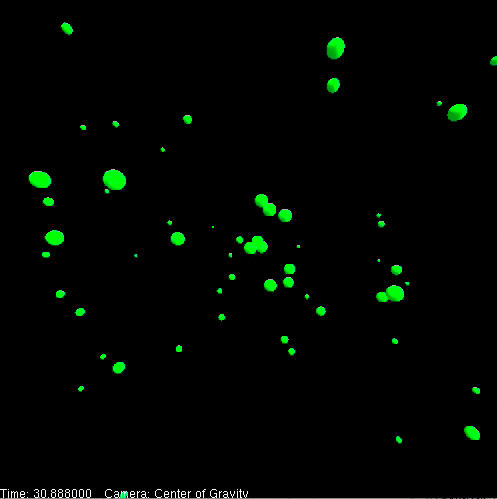
\includegraphics[width=0.5\textwidth]{chapter_whatitis_fig/simulator.png}
\caption{Screenshot of the \RSS running a simulation}
\label{WII:fig:simulator}
\end{figure}
For better observing the robots' movements the User Interface provides different camera modes: 
\begin{quote}
\begin{itemize}
	\item the \texttt{CogCamera}, where the camera is located at the center of gravity of all robots
	\item the \texttt{FollowSwarmCamera}, where the camera moves such that the swarm is always visible
	\item the \texttt{MoveableCamera}, where the user can move the camera's position by mouse or keyboard interactions
\end{itemize}
\end{quote}
More features of the User Interface will be described in Section~\ref{WII:sec:features}.\medskip

\subsection{Portability}
Besides its simple usage the \RSS stands out in its portability: it comes as executable for Windows, Linux and Mac OS X.
We also payed attention that the external libraries we used are also portable to all of these systems. Thus, the development of the \RSS is possible on Windows, Linux and Mac OS X. In addition to theses three systems, it is also easy to port the \RSS to  other UNIX-like operating systems.


\subsection{Simple Adding of New Robot Algorithms}
The \RSS comes with a set of already implemented robot algorithms. Just to name a few, there are 
\textsc{LocalFlow} (Figure~\ref{WII:fig:local-flow}),
\textsc{GridPullSpin} (Figure~\ref{WII:fig:gridpullspin2d}),
\textsc{MovingChain} (Figure~\ref{WII:fig:moving-chain}) or
\textsc{Lattice2DRobot} (Figure~\ref{WII:fig:cloning-movement}).\\

\begin{figure}[ht]
	\centering
	\begin{minipage}[t]{0.46\textwidth}
		\centering
		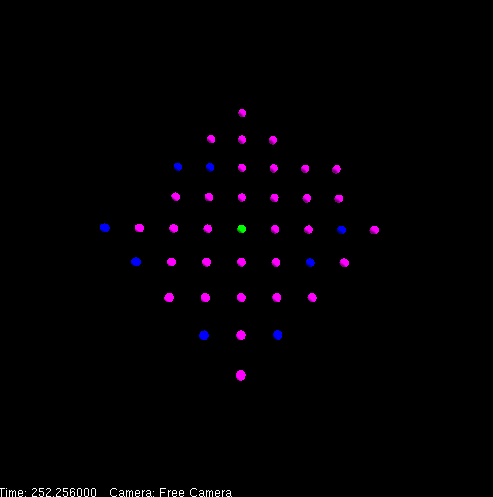
\includegraphics[width=\textwidth]{chapter_whatitis_fig/local-flow}
		\caption{Visualization of the \textsc{LocalFlow} algorithm}
		\label{WII:fig:local-flow}
	\end{minipage}$\quad$
	\begin{minipage}[t]{0.46\textwidth}
		\centering
		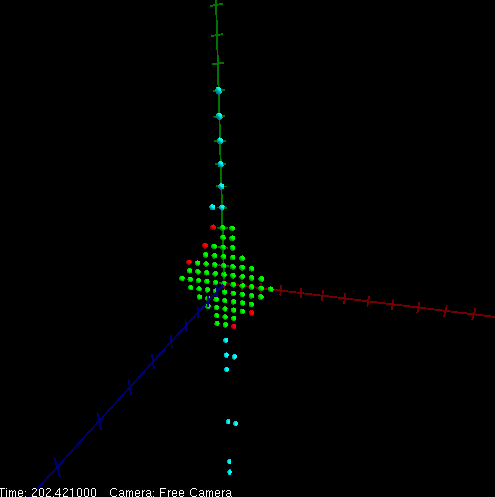
\includegraphics[width=\textwidth]{chapter_whatitis_fig/gridpullspin2d.png}
		\caption{Visualization of the \textsc{GridPullSpin} algorithm with global coordinate system displayed}
		\label{WII:fig:gridpullspin2d}
	\end{minipage}
	\begin{minipage}[t]{0.46\textwidth}
		\centering
		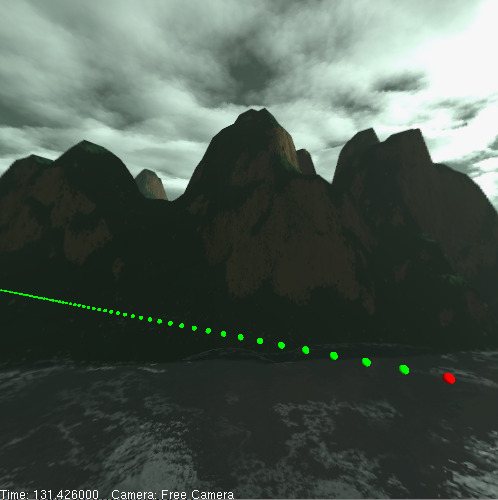
\includegraphics[width=\textwidth]{chapter_whatitis_fig/moving-chain.png}
		\caption{Visualization of the \textsc{MovingChain} algorithm with a textured skybox}
		\label{WII:fig:moving-chain}
	\end{minipage}$\quad$
	\begin{minipage}[t]{0.46\textwidth}
		\centering
		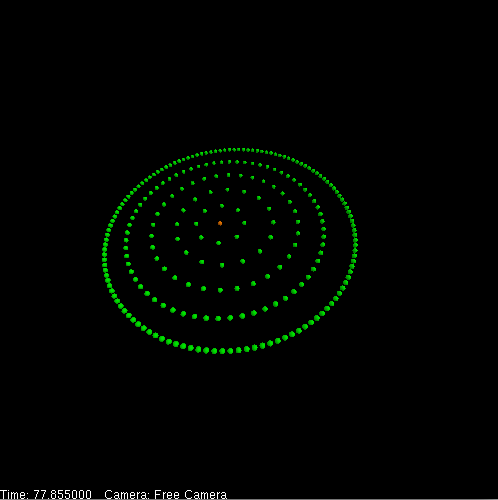
\includegraphics[width=\textwidth]{chapter_whatitis_fig/cloning-movement.png}
		\caption{Visualization of the \textsc{CloningMovement} algorithm}
		\label{WII:fig:cloning-movement}
	\end{minipage}
\end{figure}

But the \RSS is not limited to the predefined robot algorithms. It is easy to add own, new robot algorithms. This can be done by implementing the robot algorithm you want to test in \Cpp or in \Lua. 
In both cases you do not have to work through the whole code or know how the simulator works inside. Thus, you can easily add your new algorithm in just a few minutes to the \RSS.
Section~2.4 of the \RSS's User's Guide provides more information about how to add your own algorithm to the \RSS.

\subsection{Diversity of Useful Features}\label{WII:sec:features}
Besides its simple usage, the computation of statistical measures is a powerful feature of the \RSS. 
If the computation of statistical measures is enabled by the command that runs the \RSS, the statistics defined in the main project file will be generated during the simulation.
There are several supported statistics like average position of the robots, minball center of the robots, minball radius of the robots or maximal distance from the origin, just to name a few. It is also easy to extend the statistics module of the \RSS to support even more statistical measures.
Furthermore, the statistics module of the \RSS is highly adaptable. For instance, one can define, which values will be outputted during a simulation.
\par
For a clear interpreting of the statistical measures or directly inserting the result into a paper, the \RSS provides an automatic generation of GnuPlot charts of the computed measures.\medskip

As already mentioned above, the User Interface of the \RSS provides some further controlling and visualization features. 
The controlling features include the possibility to let the user pause (and resume) the simulation at any time or increase (or decrease) the simulation speed. If an according camera mode is selected (which can as well be done by the user during the simulation) the user is also able to navigate through the scene by mouse or keyboard. \par
The visualization features include some useful presentation possibilities for getting more information. Just to name a few, some of these features are
\begin{itemize}
	\item display the center of gravity of the swarm (Figure~\ref{WII:fig:cog})
	\item display a help screen providing available shortcuts (Figure~\ref{WII:fig:help-screen})
	\item display global or local coordinate systems (Figure~\ref{WII:fig:gridpullspin2d}, Figure~\ref{WII:fig:local-coordinates})
	\item display visibility graph (Figure~\ref{WII:fig:visibility-graph})
	\item single step mode
	\item save current simulation
\end{itemize}
All these features can easily be enabled by shortcuts, which can be displayed in a help screen by simply pressing \texttt{h}.


\begin{figure}[ht]
	\centering
	\begin{minipage}[t]{0.46\textwidth}
		\centering
		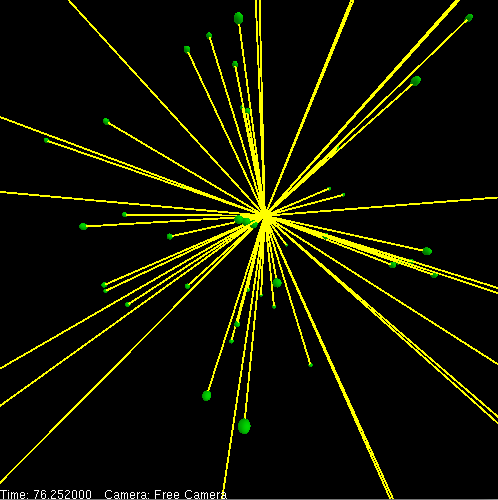
\includegraphics[width=\textwidth]{chapter_whatitis_fig/cog.png}
		\caption{Center of gravity of the swarm}
		\label{WII:fig:cog}
	\end{minipage}$\quad$
	\begin{minipage}[t]{0.46\textwidth}
		\centering
		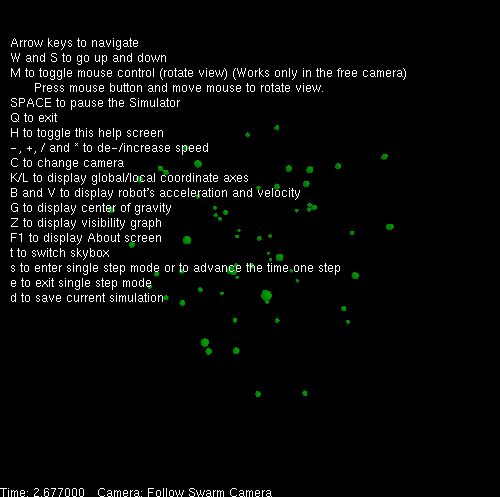
\includegraphics[width=\textwidth]{chapter_whatitis_fig/help-screen.png}
		\caption{Help screen of the \RSS}
		\label{WII:fig:help-screen}
	\end{minipage}
	\begin{minipage}[t]{0.46\textwidth}
		\centering
		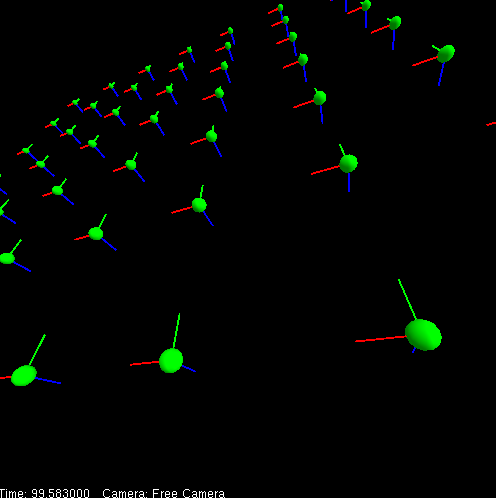
\includegraphics[width=\textwidth]{chapter_whatitis_fig/local-coordinates.png}
		\caption{Local coordinate systems}
		\label{WII:fig:local-coordinates}
	\end{minipage}$\quad$
	\begin{minipage}[t]{0.46\textwidth}
		\centering
		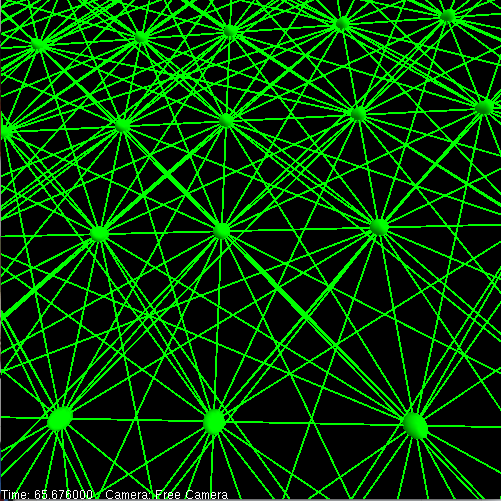
\includegraphics[width=\textwidth]{chapter_whatitis_fig/visibility-graph.png}
		\caption{Visibility graph of robots arranged in a lattice}
		\label{WII:fig:visibility-graph}
	\end{minipage}
\end{figure}


\section{Application Possibilities}\label{WII:sec:application}
In this section we will give some ideas in which areas the \RSS can be a very helpful tool.\par
Imagine, you developed an robot algorithm and want to get an idea of the robots' movement.
Of course, you could run through your algorithms step by step by using only pen and paper. But for a higher number of robots or iterations this procedure becomes labor-intensive or even infeasible. At this point the \RSS gets into the game. After you have implemented your robot algorithm you can see the behavior of an (almost) arbitrary large number of robots in an (almost) arbitrary high number of iterations. Thus, the \RSS gives you deeper insights and intuition about your algorithms.
Another advantage of the \RSS against the pen and paper method is the visualization of algorithms in 3D which can become very cumbersome with pen and paper. Moreover you can easily display additional visual information like the visibility graph, the center of gravity or movement vectors.\par
If you do not only want to observe the robots movement, but get an idea of the running time or some other measures of your algorithm, the statistical computations of the \RSS can deliver you good hints for the theoretical analysis of your algorithm.\par
Furthermore you can often simply verify with the \RSS, whether your algorithm works (at least in practice).


	
\chapter{Simulator Design and Reference}
\label{chap:IG}

\section{Introduction}\label{SG:sec:introduction}
\begin{quote}
	\textit{Thus spoke the master programmer:\\
	After three days without programming,\\
	life becomes meaningless.}\\[2mm]
	(The Tao of Programming)\medskip	
\end{quote}


\noindent
How to design a complex software in a matter of months? That was the question the project group was facing at the meeting in Schloss Gehrden in November. Even worse: How to design a complex software capable of running on \emph{all three} major operating systems with a group of developers who had \emph{never} worked together before and who had a multitude of different backgrounds and skill levels?\smallskip

\noindent
In the first meetings it became clear that one important aspect of the answer to these questions was to keep the Simulator simple in some areas while still retaining the ability to simulate most important theoretical models.
We deliberately decided to keep the user interface as simple as possible and to keep the simulation itself event-based (as opposed to continuous). We also decided to not allow any user interaction with the simulation itself at runtime. Together these decisions allowed us to make a few simplifying assumptions which kept the complexity of the software manageable.\smallskip

\noindent
The second important principle was that the simulator had to be useful to our theoretical research. It should be able to support all major theoretical models with regard to the time model, the accuracy of robot movements and local views. Since we could not possibly anticipate which models would be used we needed to keep the simulator as extensible and as modular as possible. The one major restriction with regard to the theoretical model we made was that we committed to the \emph{\Look-\Compute-\Move} model which we only slightly generalized to a \emph{\Look-\Compute-\HandleRequests} model where the robots are able to formulate general requests to change their environment. Except for this restriction we tried to make the simulator as extensible as possible and provided easy ways to implement new models for time, local views and request--handling. Later in development we also implemented a way to dynamically load robot algorithms without recompiling the simulator using the script language Lua \cite{reference:Lua}.\smallskip

\noindent
Since it was always clear that the simulator should only be a tool for our theoretical research it had to be developed fast. This lead to a very agile design process in which the first step was to roughly define concrete modules and their interfaces which allowed us to split our project group in subteams of $2$--$4$ members, each responsible for a certain module or submodule. Keeping the size of the subteams small allowed for a rapid development cycle within each subteam. To improve the communication between subteams each individual in the project group was part of two subteams which simplified communication between subteams greatly since each subteam had direct access to the members of many other subteams. Within the subteams a more detailed and elaborate specification of the modules and submodules was done (often in parallel to the actual implementation by solving design problems as they came up).\smallskip

\noindent
To help the subteams in their process and to smooth out the skill differences between their members a small series of lectures on topics such as boost, unit testing and our bug tracking tool was organized. A mandatory code style guideline was adopted based on the Google Code Styleguide \cite{reference:Google}. We also tried to make unit testing as easy as possible by using the boost unit test framework and providing some infrastructure to the testing process (though the decision whether to use unit testing was ultimately left to each subteam). We used CMake \cite{reference:CMake} to build the \RSS on a multitude of different IDEs and operating systems. The most important factor in the success of the \RSS was, however, the good communication structure between the subteams which minimized interface problems and made the unique skill set of each team member available where it was needed most.\smallskip

\noindent
In the next sections we will try to give an overview over the design of the \RSS and try to provide some insight into why it is designed and implemented the way it is. Section~\ref{IG:sec:overview} gives a rough overview over the overall design and the general structure of the simulator. The different threads and their synchronization are described in Section~\ref{sec:synchronization}. A detailed overview over the \module{SimulationKernel} and \module{Visualizer} modules is given in Section~\ref{sec:simulationkernel} and Section~\ref{sec:visualizer} respectively. Finally Section~\ref{IG:sec:odds} shares some interesting statistical data about the development process of the \RSS. Naturally a document such as this cannot aim for completeness and while it is our goal to give the reader a somewhat in--depth description of the \RSS there have been some omissions, most notably the way Lua is used within the simulator and how parsing project files is accomplished. 

\section{Overview and Modularization}\label{IG:sec:overview}

This section gives a rough overview about the structure and basic organization of the \RSS which will be explored in more detail in later sections. The simulator is divided into the following main modules:
\begin{itemize}
\item \module{SimulationKernel}
\item \module{Visualizer}
\item \module{SimulationControl}
\end{itemize}

\noindent
Seen from a very high level, the \module{SimulationKernel} does the actual simulation and produces \class{TimePoint} objects while doing so. The \class{TimePoint} stores a complete state of the simulation for a given time and, additionally, statistical information about the state. The visualizer takes \class{TimePoint} objects and visualizes them in some form (currently using OpenGL and GLUT). It also handles user input. \class{SimulationControl} controls how the simulation is executed. It is responsible for handling changes in simulation speed (including pausing) and checking termination conditions. \smallskip

\noindent
Figure~\ref{fig:modularization} depicts the relations between the different modules. Note that the given attributes and methods describe not the complete interfaces of the modules, but only the interface needed for inter--module communication. See Appendix~\ref{sec:classlist} for a complete description of the most important module/class interfaces.\smallskip

\begin{figure}
\centering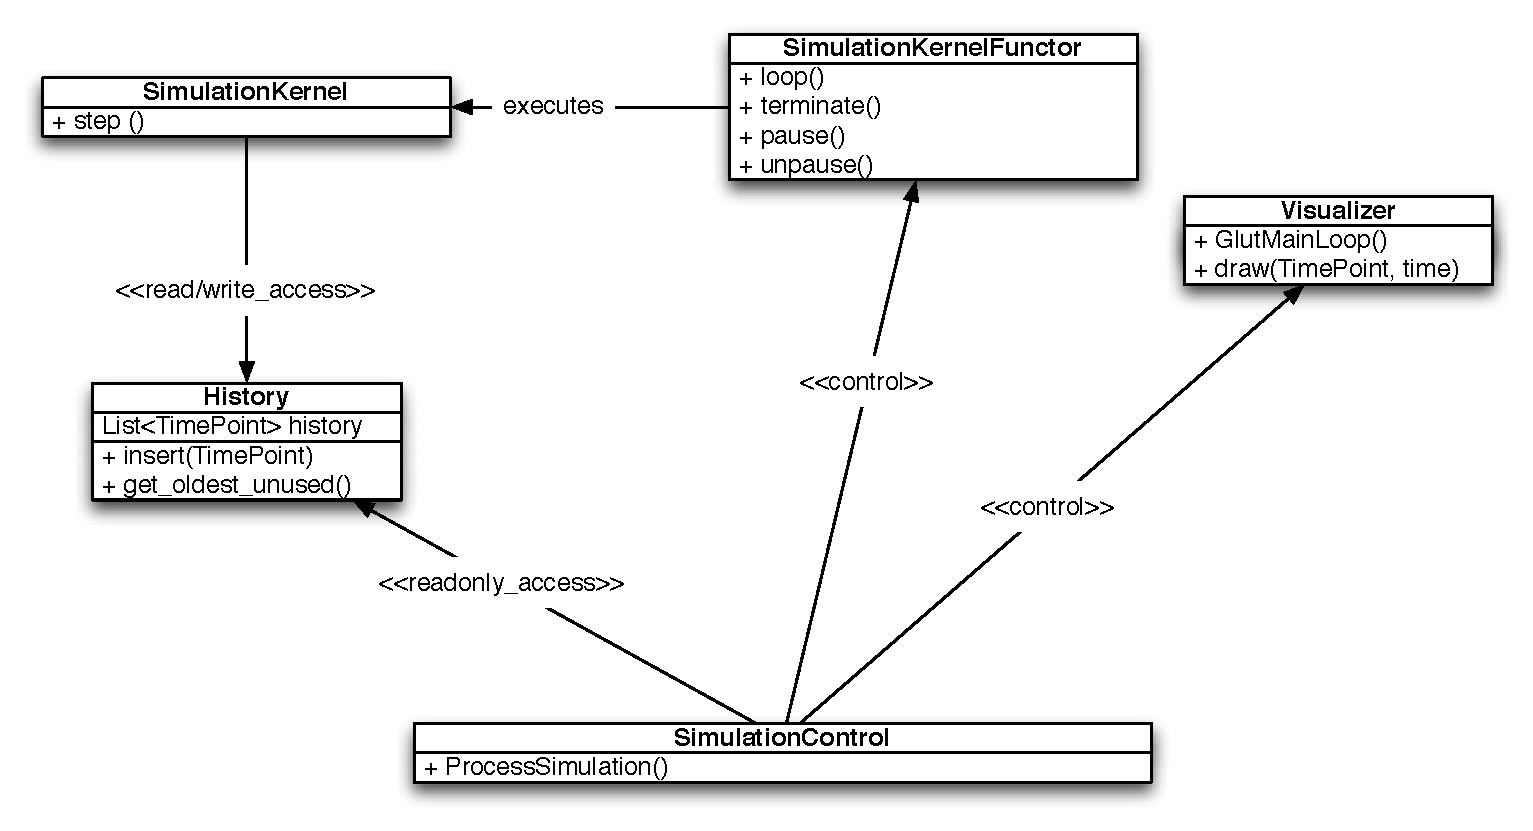
\includegraphics[width=0.85\linewidth]{chapter_reference_fig/modularization}
\caption{Modularization of the \swsim}\label{fig:modularization}
\end{figure}

\noindent
Visualizing and simulating is done in two different threads. This has multiple advantages the most important being that we can make a clear distinction between simulation time and visualization time which allows the user to adjust the latter while the simulation continues in the background at a high speed. The first thread is responsible for the visualization, and the control of the simulation including handling user input. This thread will henceforth be called the \emph{Control--Thread}. The second thread is responsible for doing the actual simulation itself. We will henceforth call this thread the \emph{Simulation--Thread}.\smallskip

\noindent
The central class in our design is the \class{SimulationControl} class which controls how \module{SimulationKernel} and \module{Visualizer} interact. For this there are two helper classes: The \class{History} which stores a history of the last $m$ \class{TimePoints} produced by the simulation and the \class{SimulationKernelFunctor} which executes the simulation in an endless loop but can be controlled by \class{SimulationControl}. In order to visualize time points the \class{SimulationControl} copies them from the \class{History} and forwards that copy to the \module{Visualizer}'s draw method. This design achieves a high degree of modularization with very thin interfaces between the main modules. Especially the visualizer is easily exchangeable should we decide to abandon OpenGL in the future (in fact it is also possible to execute the simulation without any visualization at all). 

\section{\module{SimulationControl} and Synchronization}\label{sec:synchronization}

This section describes the interaction between the \emph{Simulation--Thread} (covering \module{SimulationKernel}) and the \emph{Control--Thread} (covering \module{SimulationControl} and \module{Visualizer}). Any thread handling is done inside \module{SimulationControl}. It has access to the \emph{Simulation--Thread} via the \class{SimulationKernelFunctor} which provides methods to terminate, pause and resume the current simulation. The thread--safe access to shared data objects (i.e. the history object owned by \module{SimulationControl}) is synchronized by corresponding accessor methods in the \class{History} class itself (see Section~\ref{sec:history_class}).

\subsection{Notions of Time}
We will distinguish two notions of time: the \emph{Simulation--Time} and the \emph{Processing--Time}\footnote{Think of this as a kind of \emph{Visualization--Time}, i.e. the currently visualized moment in time. We did not call it so, because we do need this time--notion also in the case that there is no visualization performed.}. The Simulation--Time corresponds to the time--steps of the simulation inside the \module{SimulationKernel} (in the Simulation--Thread). The Processing--Time describes the time we are currently processing inside the Control--Thread. One time step in the Simulation--Time corresponds to a fixed (configurable) amount $\Delta$ of Processing--Time. The Processing--Time should pass proportional to real--world time\footnote{At least in between two simulation events. We may be blocked if we reach the time of an simulation event because there not yet any unconsumed world states to process. If this is the case, no Processing--Time passes until we find a new unconsumed \class{TimePoint} object.}. A point $t$ in Processing--Time corresponds to time step $t/\Delta$ in Simulation--Time.\smallskip

\noindent
We have to make sure that Simulation--Time and Processing--Time do not differ by "too much". This is needed because we will save the simulation state only for a fixed number of past events. Thus, if the Simulation--Time passes too fast (or more exactly, if we have to save too many past world states), it may happen that we overwrite the world state for a not yet processed (e.\,g. visualized) point in Processing--Time. Similar problems appear if Simulation--Time passes too slow compared to Processing--Time. To avoid such problems, we will provide some kind of synchronization in special accessor methods of the \class{History} class. See Section~\ref{sec:history_class} and the class reference in Appendix~\ref{sec:classlist}.

\subsection{History Class}\label{sec:history_class}
The history holds a buffer to a certain number (maybe all, but at least two) of past simulation states. It is accessed by both threads, therefore we need some kind of synchronization.\smallskip

\noindent
The Control--Thread accesses the history only via the \method{get\_oldest\_unused} method which \emph{consumes} the oldest \class{TimePoint} inside the history (without deleting it). The Simulation--Thread \emph{produces} \class{TimePoint} objects using the \class{History}::\method{insert} method. Producing or consuming \class{TimePoint} objects is guarded by two semaphores (using the \href{http://en.wikipedia.org/wiki/Producer-consumer_problem}{Producer--Consumer Pattern}). There are also a number of utility accessor methods which can be called from the Simulation--Thread. These are \emph{not} protected and do not change the history in any way.

\subsection{Synchronization between Simulation-- and Processing--Time}\label{sec:time_synchronization}
The two methods \class{History}::\method{insert} and \class{History}::\method{get\_oldest\_unused} make sure that Simulation-- and Processing--Time do not differ too much. In the the Control--Thread, we hold at least two successive \class{TimePoint} objects $w_i$ and $w_{i+1}$ corresponding to (Simulation--) time steps $t_i$ and $t_{i+1}$. It holds that the current Processing--Time $T_p$ lies in the (Processing--) time interval $[t_i\Delta,t_{i+1}\Delta]$.
\begin{itemize}
	\item A call to \method{insert} from \class{SimulationKernel} in the Simulation--Thread proceeds the Simulation--Time to the time--step $t_{i+2}$ of the next event by inserting a corresponding \class{TimePoint} object into the history. It blocks if this insertion would overwrite a not--yet consumed history--entry (Simulation--Time is stopped).
	\item A call to \method{get\_oldest\_unused} is issued when processing time reaches $t_{i+1}\Delta$. It returns a full copy $w_{i+2}$ of the next \class{WorldInformation} object for (Simulation--) time step $t_{i+2}$. If this call blocks, no processing time passes. Only when this call returns, the processing time continues at time $t_{i+1}\Delta$ and the (Processing--) time interval $[t_{i+1}\Delta,t_{i+2}\Delta]$ is processed.
\end{itemize}

\section{\module{SimulationKernel}}\label{sec:simulationkernel}

This section describes how the simulation itself works. Subsection~\ref{SG:sec:overview} gives a basic overview about the most important functionality while the subsections~\ref{sec:model} to \ref{sec:statistics} describe the submodules in more detail.

\subsection{Overview}\label{SG:sec:overview}

The \module{SimulationKernel} manages the actual simulation of a given scenario. In order to simplify the development of the \RSS somewhat we decided to implement an event--based discrete time simulation. This kind of simulation is still able to cover the vast majority of all theoretical models we investigated. The timing of the model is driven by the \class{ActivationSequenceGenerator} which produces a sequence of \class{Events} which each have an associated time. As already noted in Section~\ref{SG:sec:introduction} we restricted ourselves to a basic \emph{\Look-\Compute-\HandleRequests} model which means that there are exactly three kinds of events. Each event may apply to an arbitrary subset of robots in the simulation (though in practice all used time models guaranteed that each individual robot received events in the order \emph{\Look} then \emph{\Compute} then \emph{\HandleRequests}).\smallskip

Events are passed into the \class{EventHandler} which handles them. While the handling for \emph{\Look} and \emph{\Compute} events is straightforward the handling of \emph{HandleRequest} events requires that (depending on the theoretical model considered) different \class{RequestHandlers} are used. In order to be able to support as many different theoretical models as possible we decided to follow a modular approach which allows for the adding of different Event--Handling--, Time-- and View--Models. The principal classes for this are the abstract classes \class{ActivationSequenceGenerator}, \class{View} and the class \class{EventHandler} which offers support for different \class{RequestHandler} classes.

\begin{figure}
	\centering
	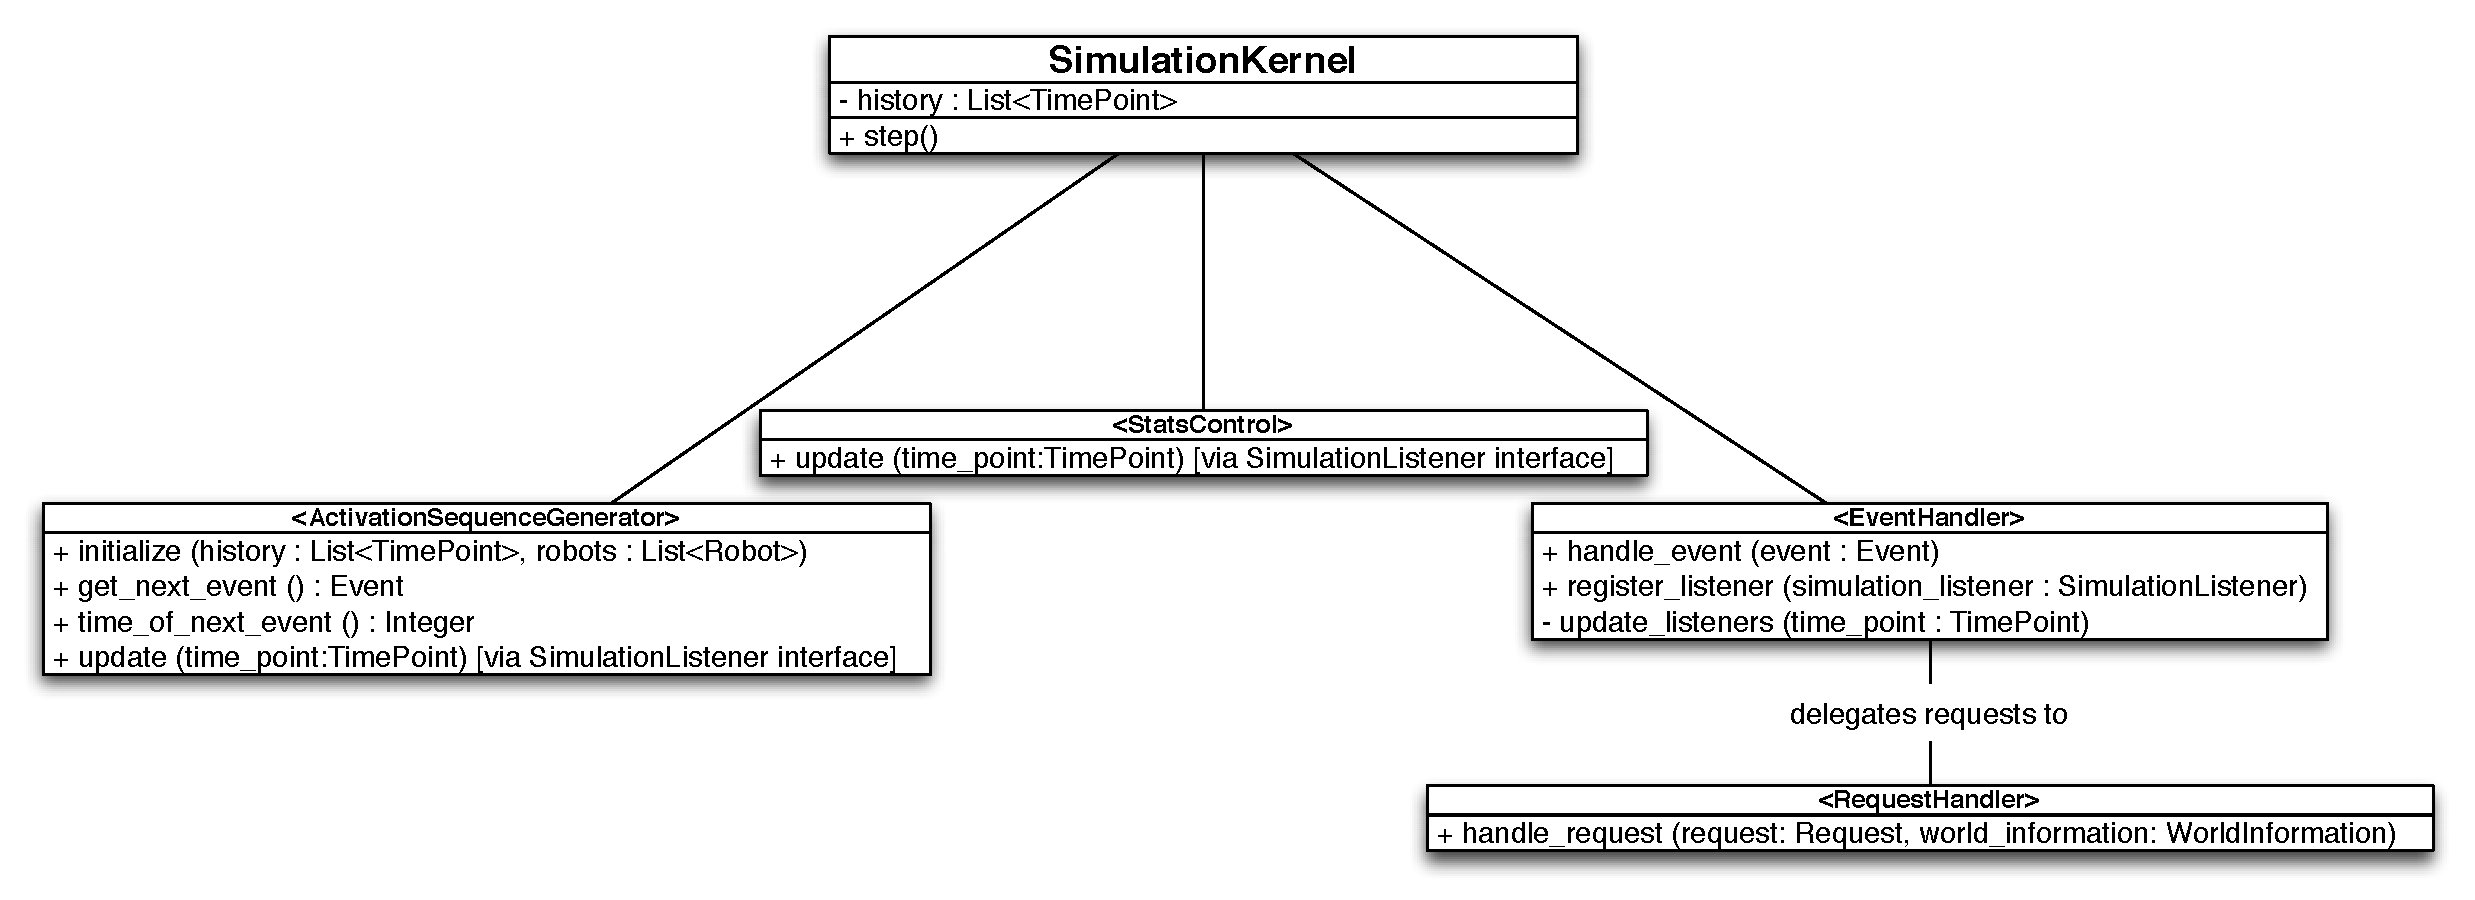
\includegraphics[width=0.9\linewidth]{chapter_reference_fig/simulation_kernel_overview}
	\caption{Overview over the \module{SimulationKernel}}\label{fig:simkernel_overview}
\end{figure}

\noindent
Figure~\ref{fig:simkernel_overview} shows a high level overview over the \module{SimulationKernel}. For each step the \class{ActivationSequenceGenerator} produces an \class{Event} which is passed to the \class{EventHandler} which handles it. This produces a new \class{TimePoint} object, which is later inserted into the \class{History} by the \class{SimulationKernel}. After producing the new time point the \class{EventHandler}
also informs all \class{SimulationListeners} (e.\,g. \class{StatsControl} and \class{ActivationSequenceGene\-rator}). Thus the implementation of the \texttt{step()} method becomes very easy and is given for reference here:

\begin{lstlisting}
void SimulationKernel::step() {
	// create a new time point
	boost::shared_ptr<TimePoint> time_point(new TimePoint());

	// fill time point
	event_handler_->handle_event(asg_->get_next_event(), *time_point);

	// insert time point
	history_->insert(time_point);
}
\end{lstlisting}

\noindent
In the following sections we will describe in more detail the world model we used (Section~\ref{sec:model}), how event producing and handling are implemented (Section~\ref{sec:events}), how different view models are realized (Section~\ref{sec:views}) and how statistics are computed (Section~\ref{sec:statistics}).

\subsection{Model} \label{sec:model}

\begin{figure}
	\centering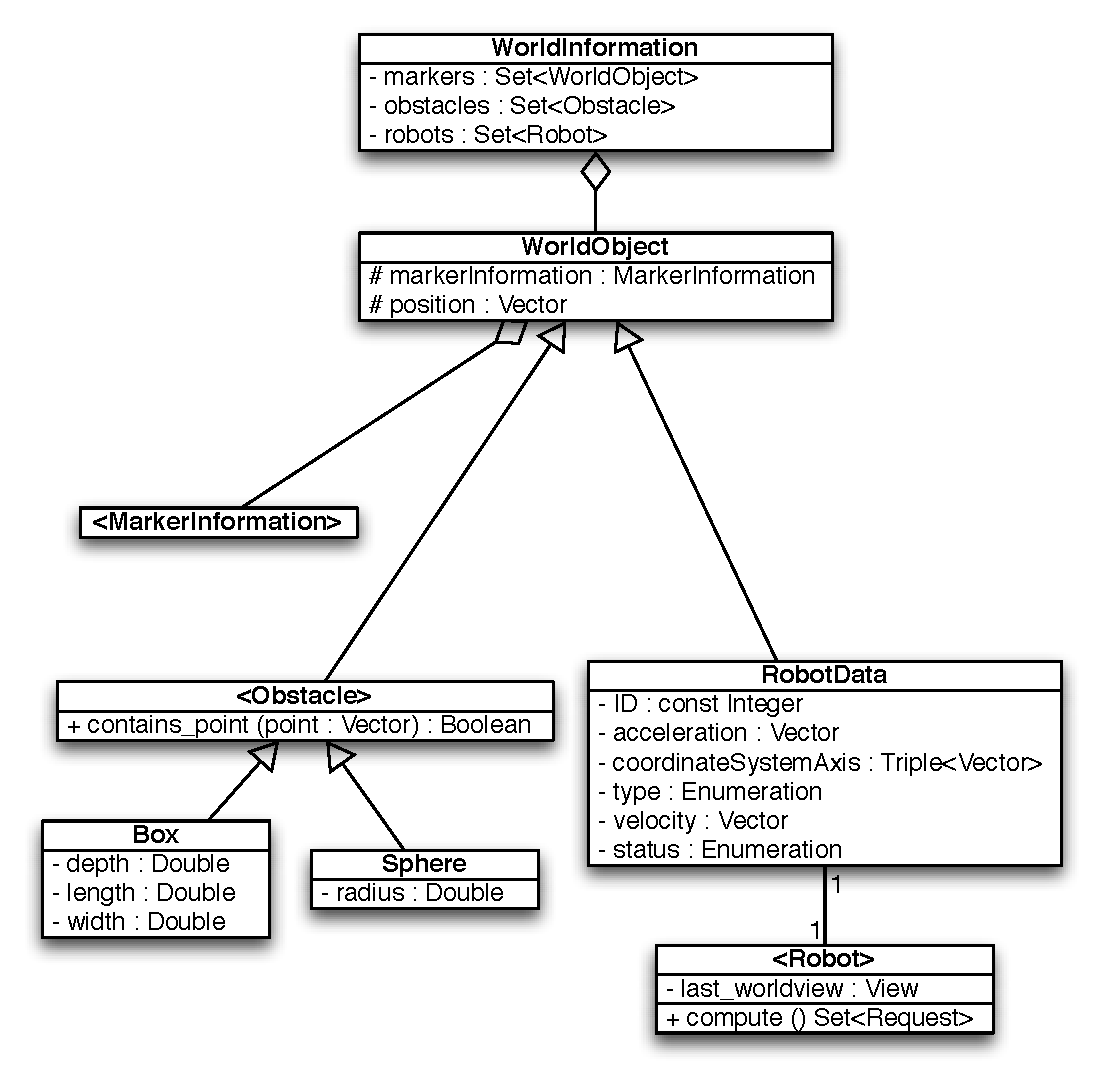
\includegraphics[width=0.75\linewidth]{chapter_reference_fig/model}
	\caption{Overview over the world model}\label{fig:model_overview}
\end{figure}

\noindent
Figure~\ref{fig:model_overview} gives an overview of the model we used. The basic entity of our model is a \class{WorldObject} which has a position in threedimensional space. Additionally information can be attached to a \class{WorldObject} with a \class{MarkerInformation} object (this was not commonly used in practice). A \class{WorldObject} may be a simple \class{WorldObject} (basically a marker floating in threedimensional space), an \class{Obstacle} or a \class{RobotData} object. \smallskip

\class{RobotData} objects represent all information about a \class{Robot} for a given time (as time advances more \class{RobotData} objects are produced for the same \class{Robot}). The fields given in Figure~\ref{fig:model_overview} represent only the most important data associated with a \class{RobotData} object (For all fields read Appendix~\ref{sec:classlist}). Each \class{RobotData} object also points to a \class{Robot} object which represents the actual robot. The \class{Robot} class is an abstract class which has a \texttt{compute} method which can be implemented by subclasses to make the robot execute a given algorithm. A robot cannot directly access the data in its \class{RobotData} objects but has to access data by using a \class{View} object (more on views in Section~\ref{sec:views}).\smallskip

The \class{Obstacle} class can be used to represent environmental obstacles in the simulation. While robots are (in most scenarios) simple points in three-dimensional space obstacles can be either spheres or boxes which occupy a volume in space. More complicated obstacle shapes can be formed by combining several obstacle objects. Since, in practice, obstacles were not commonly used in our theoretical research we do not support any inherent handling (like collision--detection) for the interaction between robots and obstacles. (However, given the need to analyze such a scenario, this could be easily added by introducing a new \class{Requesthandler}.)

\subsection{Time Models and Event Handling} \label{sec:events}

In this section we describe the support for event handling and time models and give a short list of models that have been implemented. In general the \emph{time model} defines what events are produced in which order. As noted before there are three different kinds of events: 
\begin{description}
\item[\class{LookEvent}:] A subset of the robots computes a new View
\item[\class{ComputeEvent}:] A subset of the robots executes its algorithm and computes new \class{Requests}. A \class{Request} is a general way for a robot to request a change in its environment (For example: a \class{MoveRequest} requests to change the robot's position.). \class{Requests} will be described in more detail later in this section.
\item[\class{HandleRequestEvent}:] The requests of a subset of robots are handled.
\end{description}
All events carry the time at which they happen in Simulation--Time and the subset of robots to which they apply.

\subsubsection{Time Models and the \class{ActivationSequenceGenerators}}

Events are produced by \class{ActivationSequenceGenerators}, also called ASGs, by the method \texttt{get\_next\_event()} (For a full description of the ASG interface see Appendix~\ref{sec:classlist}). The main task of an ASG is to determine in which order what kind of events should be produced. Since a theoretical worst-case adversary as used in most theoretical proofs is not easily implementable for most algorithms, we choose to implement a variety of randomized ASGs (all ASGs use the Mersenne Twister \cite{reference:mersenne} random number generator). At this time the following ASGs have been implemented:

\begin{description}
\item[\class{SynchronousASG}:] Produces events in the fixed order look, compute, move. All events apply to all robots. For every timestep a complete \LCM cycle is produced.
\item[\class{AtomicSemisynchronous ASG}:] Produces events in the fixed order look, compute, move. All events apply only to exactly one robot which executes a full \LCM cycle. For every timestep a complete \LCM cycle is produced.
\item[\class{FairAtomicSemisynchronousASG}:] Produces events in the fixed order look, compute, move. All events apply only to exactly one robot which executes a full \LCM cycle. For every timestep a complete \LCM cycle is produced. In addition to the atomic semi-synchronous ASG, the fair atomic semi-synchronous ASG divides times into cycles of length $n$, where $n$ is the number of robots. Each robot is guaranteed to be activated exactly once in each cycle.
\item[\class{AsynchronousASG}:] Produces events in no fixed order and in randomized time intervals. Each event applies to a random subset of the robots (but the ASG guarantees that each individual robot will get events in the order look, compute, move) 
\end{description}

\subsubsection{Event Handling and the \class{RequestHandlers}}

To be able to make changes to their environment robots formulate so called \class{Requests} which are computed in their \texttt{compute()} method. At this time the following types of requests have been implemented:

\begin{description}
\item[\class{PositionRequest}:] The robot requests to change its own position to the given coordinates in its local coordinate system.
\item[\class{VelocityRequest}:] The robot requests to change its own velocity to the given vector in its local coordinate system.
\item[\class{AccelerationRequest}:] The robot requests to change its own acceleration to the given vector in its local coordinate system.
\item[\class{MarkerRequest}:] The robot requests to change its own marker information.
\item[\class{MarkerChangeRequest}:] The robot requests to change the marker information of a given \class{WorldObject}.
\item[\class{TypeChangeRequest}:] The robot requests to change its own type.
\item[\class{ColorChangeRequest}:] The robot requests to change its color. This is used in visualization to display different states and behaviors in robots.
\end{description}

\noindent
Each requests carries the robot that issued it and the desired state the robot wants to achieve (e.\,g. the new position). For a detailed overview over the request classes see Appendix~\ref{sec:classlist}.\smallskip


\noindent
Requests are carried into the \class{EventHandler} by \class{Handle\-Requests\-Events}. The major design goal at this point is to ensure that a user can easily specify how each kind of request is handled. Since the number of requests is relatively small and we did not plan on adding many new request types (in fact only the \class{ColorChangeRequest} was added after the initial implementation phase was over) we decided to let the user specify a \class{RequestHandler} for each kind of \class{Request}. This makes the handling for the different request types completely orthogonal and allows a vast number of theoretical request--handling models. However even though request handling is orthogonal for the different request types from a theoretical standpoint, from a coding standpoint handling for certain types of requests is very similar. For this reason we introduced a common class to handle \class{PositionRequests}, \class{VelocityRequests} and \class{AccelerationRequests}, which require very similar handling due to the vector character of their corresponding values.

When a \class{Handle\-Requests\-Event} is encountered by the \class{EventHandler}, it delegates it to the appropriate \class{RequestHandler}. Usually the \class{EventHandler} has a \class{RequestHandler} for each kind of \class{Request} (If no request handler is set, the corresponding requests are simply discarded).
At this time the following \class{RequestHandlers} have been implemented:

\begin{description}
\item[\class{VectorRequestHandler}:] A generalized handler for \emph{Vector Requests} (\class{PositionRequest}, \class{VelocityRequest}, \class{AccelerationRequest}). It implements a pipeline of \class{VectorModifi\-ers} which can modify a vector in any given way (e.\,g. making it inaccurate by adding a small randomized number to each coordinate). For a complete list of \class{VectorModifiers} see Appendix~\ref{sec:classlist}.
\item[\class{CollisionPositionRequestHandler}:] A subclass of the \class{VectorRequestHandler} which supports collision detection.
\item[\class{TypeChangeRequestHandler}:] Handles type change requests by doing exactly as the robot wishes.
\item[\class{ColorChangeRequestHandler}:] Handles color change requests by doing exactly as the robot wishes.
\item[\class{MarkerChangeRequestHandler}:] Handles marker change requests by doing exactly as the robot wishes.
\item[\class{MarkerRequestHandler}:] Handles marker requests by doing exactly as the robot wishes.
\end{description}
All \class{RequestHandlers} have a certain probability $0 \le p \le 1$ to just discard a certain request (the probability can be supplied in the project file and was set to $0$ in most investigated scenarios).

\noindent
If the \class{EventHandler} encounters a different kind of event (\class{LookEvent}, \class{ComputeEvent}), much simpler handling routines are used. In case of a \class{LookEvent} for each robot in the subset carried by the event a new view is computed (more on this in Section~\ref{sec:views}). In case of a \class{ComputeEvent} all robots in the subset carried by the event execute their algorithm and compute a new set of requests which are stored in the event in order to be passed to the ASG after the \class{EventHandler} updates its listeners. In all cases handling a event causes a new \class{TimePoint} to be produced (or more accurately: it causes an empty \class{TimePoint} object, passed to the \class{EventHandler} to be filled) and stored in the \class{History} by the \class{SimulationKernel}. \smallskip

The following chapter introduces the design for the different view--models. It is quite interesting to see how basically the same goals (allow the maximum amount of theoretical models for the user while keeping coding and design complexity to a minimum) can lead to vastly different design approaches.

\subsection{Support for View Models} \label{sec:views}
This section describes how the \class{View} class is used to restrict the access of \class{Robot}s' to their own and especially others \class{RobotData} objects. The idea behind restricting the access is to realize and enforce different view models directly in the implementation. Thus, we implemented for example the class \class{CloneView} to model the view model used in our \textsc{CloningMovement} paper. This class allows the robot to access attributes of \class{RobotData} only of those robots, which are positioned inside a sphere around the querying robot --- realizing the spheric view used in the paper. The following subsection provides a detailed description of the (abstract) \class{View} class and its subclasses.

\subsubsection{The Abstract \class{View} Class and its Subclasses}
When implementing different view models two problems had to be solved: 
\begin{enumerate}
\item
	How should the common interface of all view models look like? Such an interface is needed to avoid too strong dependencies between a concrete implementation of the \method{compute} method of \class{Robot} and a concrete view model.
	
\item
	How can code duplication be avoided when implementing (only slightly) different view models?
\end{enumerate}

The first problem is solved by the abstract \class{View} class. The class provides an interface for basically every attribute of each kind of \class{WorldObject}s. For example to access the position of a robot one can use the \class{View} method \method{Vector3d get\_position(const Robot\& caller, WorldObjectRef world\_object) const}. The first parameter identifies the querying (calling) robot to enforce certain access restrictions, while the second parameter identifies the \class{WorldObject} of which the position should be returned. The other access methods have a similar signature. Note that the identifier (in this case) is an object of type \class{WorldObjectRef}, which is a typedef to \texttt{boost::shared\_ptr<Identifier>}. We use the \class{Identifier} class to identify \class{WorldObject}s without giving the robot the possibility to directly access the attributes and to thus bypass the \class{View} class. To get \class{Identifier} objects a \class{Robot} has to use one of the methods \method{get\_visible\_robots}, \method{get\_visible\_obstacles}, and \method{get\_visible\_markers} provided by the \class{View} class. 


Although we refer to the \class{View} class as an abstract class, it is technically not an abstract class. Actually, it implements all the access methods, but throws an \method{OperationNotSupported} exception in each of them. Thus, using an \class{View} object one could model a ``no view at all'' view model. Although, there is probably very limited use for such a view model, this kind of implementation allows subclasses to just override the attribute-getter-methods they would like to give access to. 


To solve the problem of code duplication when implementing the many different view models, we decided to provide default implementations for each method of the \class{View} class. Thus, we have for example a \class{PositionView} class doing nothing else but implementing the \method{get\_position} method mentioned above. More interestingly, we also provide default implementations for spheric views and neighbor views (i.e. next $k$ nearest robots are visible) using an octree as data structure to speed up the calculation. These and the other helper classes can then be used to construct the needed view model. For example for seemingly complicated view model \class{CloneView} basically looks like this:

\begin{lstlisting}
class CloneView: public virtual SphericView,
		public virtual IdView,
		public virtual TimeView,
		public virtual PositionView,
		public virtual VelocityView 
{
public:
	CloneView(double view_radius) : SphericView(view_radius) {;}
	virtual ~CloneView() {;}		
}
\end{lstlisting}

\noindent
Currently the following view models are supported:
\begin{description}
\item[\class{GlobalView}:] Robots can see everything globally.
\item[\class{RadialView}:] Robots can see everything in a given view radius.
\item[\class{SelfView}:] Robots can only see itself, but can get all information about itself.
\item[\class{ChainView}:] Every robot can see the position of $k$ neighbor robots.
\item[\class{CloneView}:] View model used in the \textsc{CloningMovement} paper (i.e. robots can see position and movement of other robots in a given view radius).
\item[\class{COGView}:] Every robot can see every other robots position, velocity and acceleration. The coordinate system and id of each robot is not visible.
\item[\class{OnePointFormationView}:] Every robot can see every other robots position, velocity and acceleration only in a limited radius.
\end{description}

\subsubsection{Assignment of the Views using \class{RobotControl}}
The \class{View} of a \class{Robot} is assigned by the so called \class{RobotControl}. \class{RobotControl} is an abstract class again. It contains only three methods: \method{update}, \method{compute\_new\_request}, \method{compute\_view}. The \method{compute\_new\_request} method is basically a wrapper for \texttt{robot.compute()}, but the \method{update} and \method{compute\_view} are pure virtual methods. The \method{update} method is called once a new \class{WorldInformation} is available and typically simply creates a \class{View} object wrapping the given instance of \class{WorldInformation}. This \class{View} object is then used in \method{compute\_view} to assign a \class{View} to a given \class{Robot}. Currently, there are only two types of \class{RobotControl}s:
\begin{description}
\item[\class{UniformRobotControl}:] \class{RobotControl} that assigns the same \class{View} to all \class{Robot}s. 
\item[\class{RobotTypeRobotControl}:] \class{RobotControl} that assigns a \class{View} depending on the robot type of the given \class{Robot} (e.\,g. \texttt{MASTER}s get \class{GlobalView} and \texttt{SLAVE}s get \class{RadialView}).
\end{description}
The concrete \class{View} subtype assigned in the \class{RobotControl} is not hardcoded inside the classes mentioned above, but chosen by an \class{AbstractViewFactory}. \class{AbstractViewFactory} is an interface having a pure virtual method \method{create\_new\_view\_instance}. The class templates \class{ViewFactory} and \class{ParametrizedViewFactory} implement this interface, where the template type is used to determine the \class{View} subclass that should be created.


\subsection{Statistics} \label{sec:statistics}

It is not always the case that all desired data can be learned by observing the visualization of a simulation of a certain scenario and sometimes a quick glance on some diagram or even a table of numeric data can provide far more insight than spending ones night watching hourlong simulations. Also for some (especially randomized) algorithms it makes sense to provide a statistically sound analysis of their behavior that just cannot be made if the only way of gaining information from a simulation is by actually watching it.\smallskip

\noindent
For these reasons we decided at an early stage in the design process to include a statistics submodule which is capable of computing and outputting various statistics in a meaningful and easily processable way.\smallskip

\begin{figure}
\centering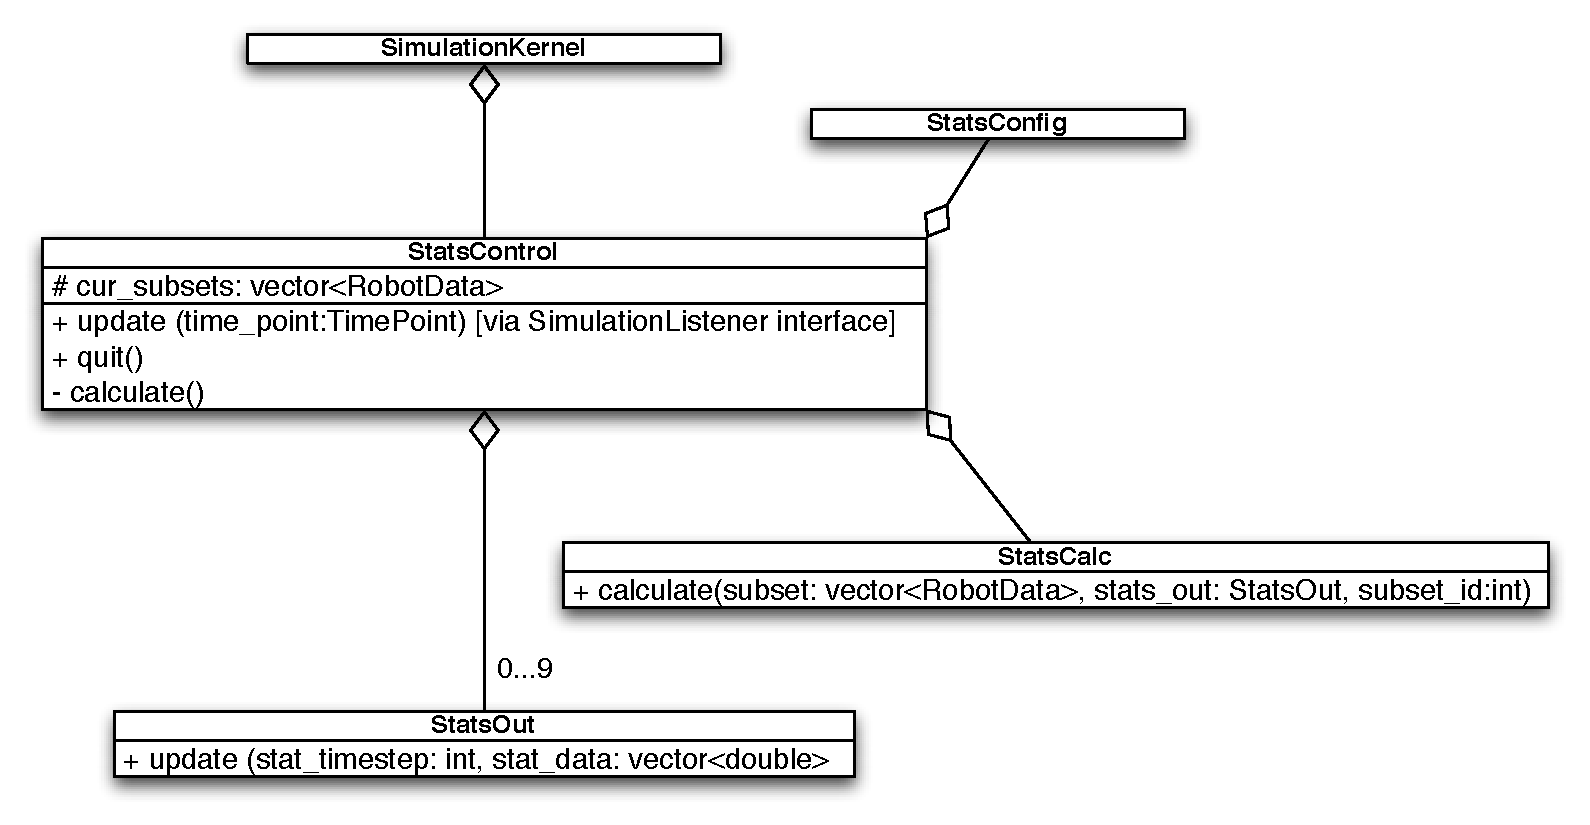
\includegraphics[width=0.78\linewidth]{chapter_reference_fig/statistics}
\caption{Statistics Module}\label{fig:statistics}
\end{figure}

Figure~\ref{fig:statistics} shows the Statistics Module. The Statistics Module calculates various statistics and logs them to GnuPlot files. The main class of the Statistics Module is the \class{StatsControl} class which implements the \class{update} method of the \class{SimulationListener} interface. This means that \class{StatsControl} is updated whenever a \class{Event} is handled and a new \class{TimePoint} is produced.\smallskip

\noindent
New statistics are calculated once for each time step (even if more than one \class{Event} is handled during that timestep). The class \class{StatsConfig}, which is initialized from parameters in the project file at startup, stores what statistics are computed for which subset of robots. At this moment the supported subsets are:
\begin{itemize}
\item All robots
\item All active robots
\item All inactive robots
\item All masters
\item All active masters
\item All inactive masters
\item All slaves
\item All active slaves
\item All inactive slaves
\end{itemize}
The supported statistics are:
\begin{itemize}
\item Number of robots in the subset
\item Number of masters in the subset
\item Number of slaves in the subset
\item Average position of the robots in the subset
\item Minball center of the robots in the subset
\item Minball radius of the robots in the subset
\item Movedistance of minball center
\item Volume Quotient of the robots in the subset
\item Maximum of all minimal distances between robots in the subset in local view
\item Maximal distance from the origin
\item Maximal $L_1$ distance from the origin
\end{itemize}

\noindent
Whenever \class{StatsControl} recalculates the statistics it invokes the \class{calculate} method of the \class{StatsCalc} object and supplies the desired subset of robots for which the statistics should be calculated. Each subset of robots is associated with a \class{StatsOut} class which is responsible for logging the statistics for that subset of robots to a GnuPlot file. Since there are $0$ to $9$ subsets of robots there are $0$ to $9$ \class{StatsOut} objects.\smallskip

\noindent
On termination of the simulation the \class{quit()} method of \class{StatsControl} is called by the \class{SimulationKernel}. \class{StatsControl} then closes all open files by calling the \class{quit()} methods of the \class{StatsOut} objects.\smallskip

\noindent
This design leads to a  Statistics Module which is easily extendable for both new kinds of subsets of robots and new statistics to compute for these subsets. (In fact new kinds of statistics were introduced multiple times in the research phase of our project group.)


\section{\module{Visualizer}}\label{sec:visualizer}

Even though a simulation without a visualization is possible and might even yield important theoretical results it is not as much fun to watch endless sequences of numbers as it is to watch actual robots in threedimensional space. For this reason (and of course because watching the execution of an algorithm provides a valuable intuition about its behavior) we included a visualization module with our \RSS. As described in Section~\ref{sec:synchronization} the visualization module is executed in the Control--Thread along with Simulation Control.\smallskip

\begin{figure}
\centering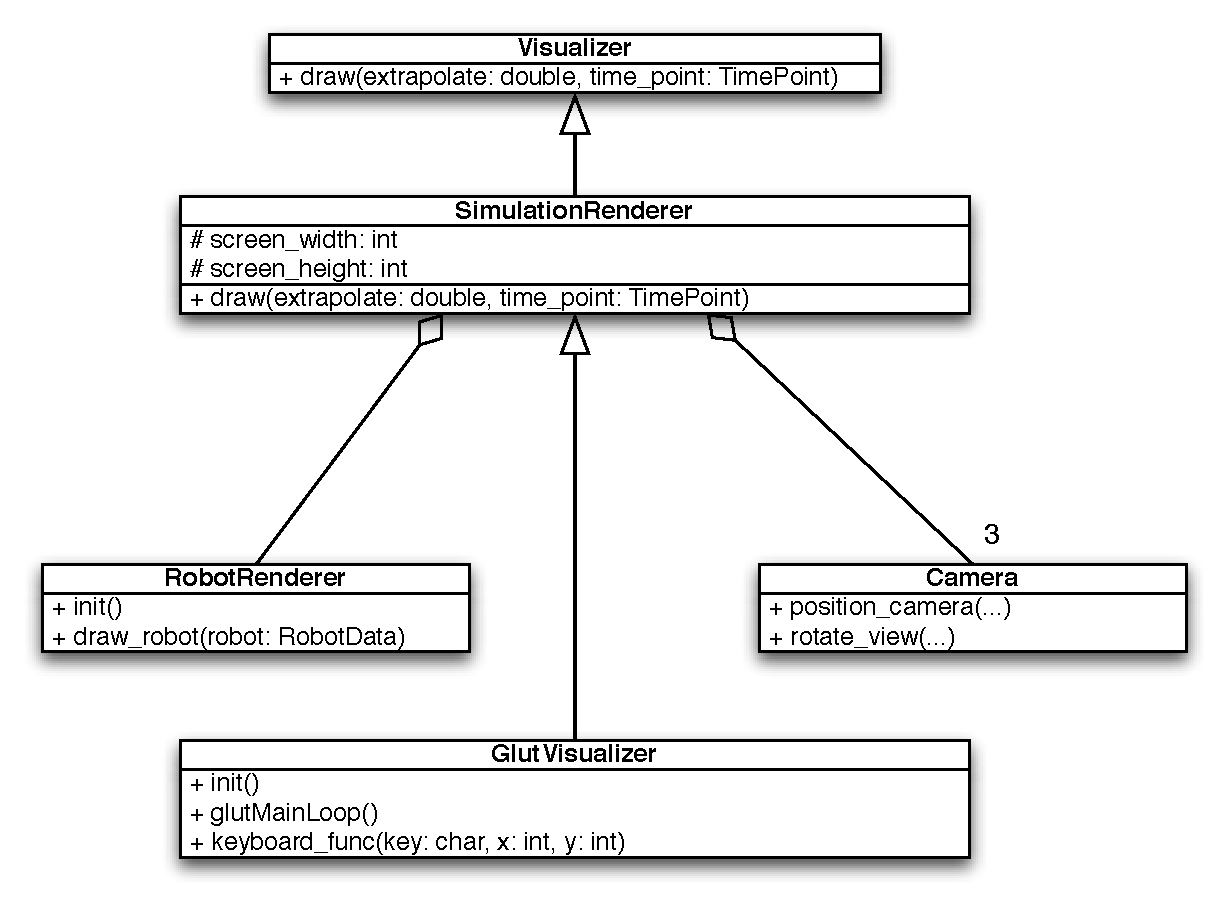
\includegraphics[width=0.75\linewidth]{chapter_reference_fig/visualizer}
\caption{Visualizer}\label{fig:visualizer}
\end{figure}

As Figure~\ref{fig:visualizer} shows, \class{GlutVisualizer}, is the central class within the \module{Visualizer} module. \class{GlutVisualizer} contains the \class{GlutMainLoop} method, which is the main method of the \emph{Control--Thread}. \class{GlutVisualizer} also contains basic methods for handling keyboard events and delegates them either to \class{SimulationControl} or the methods inherited from \class{SimulationRenderer}.
Most of the functionality of \class{GlutVisualizer} is inherited from the \class{SimulationRenderer} class which contains the functions needed to actually render the environment using the OpenGL framework. OpenGL was chosen as a rendering framework since it is easily obtainable and works on all major operating systems. Since rendering robots is more complicated than rendering the rest of the environment (\class{SkyBox}, obstacles and markers) the \class{RobotRenderer} encapsulates all functionality for this task. A number of different cameras are supported which all inherit from the abstract \class{Camera} class (The complete \class{Camera} class can be found in Appendix~\ref{sec:classlist}):

\begin{description}
\item[\class{CogCamera}:] This camera always centers on the robot swarm's center of gravity.
\item[\class{FollowSwarmCamera}:] This camera always keeps every robot in the robot swarm and every marker in the view.
\item[\class{MoveableCamera}:] This camera can be controlled by the user via mouse and keyboard.
\end{description}

\class{SimulationRenderer} implements the abstract \class{Visualizer} interface which is used by \module{SimulationControl} to call the \class{draw($\ldots$)} method. This method takes two parameters: A \class{TimePoint} to render and a double value which indicates how far this \class{TimePoint} should be extrapolated. This is necessary since the underlying simulation is discrete and produces \class{TimePoints} only for the discrete \class{Events} that occur. Interpolation between \class{Events} is therefore necessary to provide a continuous visualization (For more information about how the continuous time is derived from the discrete time of the \class{Events} see Section~\ref{sec:synchronization}).

\section{Odds and Ends}\label{IG:sec:odds}
To get an overview over how the development of the \RSS progressed over time we sometimes used StatsSVN \cite{reference:StatsSVN} which produces statistical data about the code checked into a source control system.
Since this data may offer some interesting insight into the development process of the \RSS, some of it is shared in this section.

\begin{figure}[pt]
\centering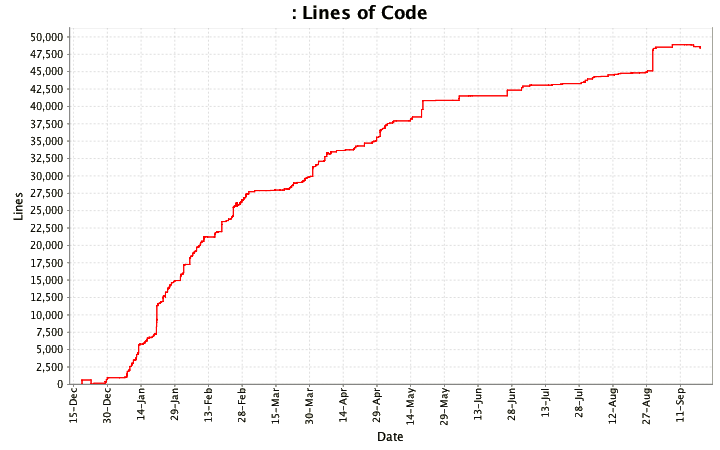
\includegraphics[width=0.75\linewidth]{chapter_reference_fig/loc}
\caption{Lines of Code over time}\label{IG:fig:loc}
\end{figure}


Figure~\ref{IG:fig:loc} shows how the lines of code in the \RSS developed over time. Development started on Christmas Eve 2008 and the main coding phase continued until the middle of March 2009. After March 2009 the theoretical work started to be the main aspect of the project group. Nevertheless there was still work on the simulator as it was adapted to the various theoretical models. In the late phase of the project group most theoretical frameworks were implemented and adjustments to the \RSS were made rather sporadically. Some work was still done (mostly to implement computational geometry algorithms) but at that time the simulator could handle the majority of scenarios investigated by the project group.

\begin{figure}[phbt]
\centering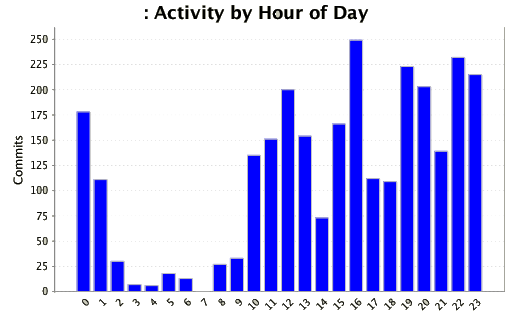
\includegraphics[width=0.65\linewidth]{chapter_reference_fig/activity_time}
\caption{Number of commits on different hours of the day}\label{IG:fig:time}
\end{figure}

Figure~\ref{IG:fig:time} shows how commits to our source control system were distributed according to the hours of the day. Most commits were made in the late morning (12:00 to 16:00) and midday (20:00 to 0:00) meaning that on a whole the project group managed to avoid the normal coding times of computer science students (2:00 to 5:00).

\begin{figure}[phbt]
\centering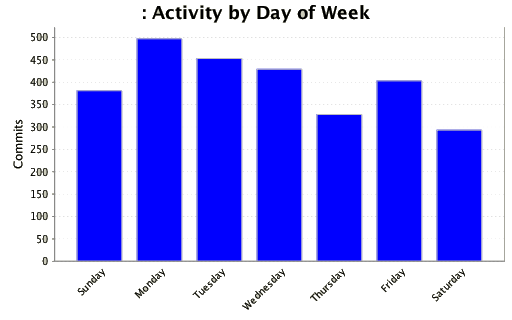
\includegraphics[width=0.65\linewidth]{chapter_reference_fig/activity_day}
\caption{Number of commits on different weekdays}\label{IG:fig:day}
\end{figure}

As Figure~\ref{IG:fig:day} shows working was pretty evenly distributed according to the days of the weeks (though this doesn't hold for the individual programmers!) with the concept of a \emph{weekend} being relatively unknown to us.\smallskip

\noindent
To conclude this section we will finish with another quotation from the \emph{Tao of Programming} \cite{reference:tao}: \smallskip

\noindent
\begin{quote}
\emph{A manager went to his programmers and told them: ``As regards to your work hours: you are going to have to come in at nine in the morning and leave at five in the afternoon.'' At this, all of them became angry and several resigned on the spot.}\smallskip

\noindent
\emph{So the manager said: ``All right, in that case you may set your own working hours, as long as you finish your projects on schedule.'' The programmers, now satisfied, began to come in at noon and work to the wee hours of the morning.}
\end{quote}
 
\newpage
\begin{appendix}
\chapter{Appendix}

\section{Design Questions} \label{sec:questions}
This appendix lists a number of design questions and their resolutions as they were encountered in the design of the \RSS. These have been copied raw from the guideline documents of the specific teams and may be outdated. Nevertheless they provide an interesting perspective in the problems and issues that we encountered when designing the simulator.

\subsection{SimulationControl}

\begin{designQuestion}\label{q:stepInvariant}
Why do we restrict the access to the \attribute{history} attribute to read--only? Write access would allow a more sophisticated user interface that allows a more interactive way of handling the simulation (e.\,g. changing robot attributes or model parameters between two steps).
\end{designQuestion}
\begin{resolution}
While it is true, that write access would provide the possibility for a more comfortable user interface, it will definitely make the module interaction much more complicated. Any change to the world state or model parameters would pose some kind of restriction to the assumption the \module{SimulationKernel} may take between two calls to \method{step}. Furthermore such changes could break data--structures inside \module{SimulationKernel}, with the need to rebuild them (consider a visibility data structure; any abrupt change to robot positions or their view radius would imply the need to rebuild them).

We should try to concentrate on the simulation itself and not on a fancy user interface. If we have completed the simulator itself and have some spare time, we could still improve the possibilities of the user interface by providing special control methods inside \module{SimulationKernel} allowing certain, well--defined changes of the world state.
\end{resolution}

\begin{designQuestion}\label{q:interpolationModule}
If we use an event--based time model, we have to provide a method to interpolate the world state between two events (for components needing to access the world state in--between two events). How should this be implemented? Possibilities include an interpolation method inside \module{SimulationKernel}, a separate interpolation module or an utility methods for interpolation.
\end{designQuestion}
\begin{resolution}
We will provide world--state interpolation (note that we mainly need linear interpolation) in form of an utility method. Such a method may be of interest in other modules as well and does not depend on any other component (except for the \class{WorldInformation} class). Anyway, we should provide some kind of \class{Utility} class gathering candidates for useful global methods.
\end{resolution}

\begin{designQuestion}
Where to implement a GUI?
\end{designQuestion}
\begin{resolution}
As indicated in Design Question~\ref{q:stepInvariant}, a fancy GUI is considered less important. Nevertheless, we need to provide some hooks where it can be placed in the overall design. We suggest the following solution:
\begin{quotation}
Implement \module{SimulationControl} as an (abstract) class with default implementations for thread handling and the set--up process. User interfaces (graphical as well as non--graphical) can be implemented as subclasses or use the class corresponding to \module{SimulationControl} to control the rest of the \swsim. Note that the visualization using OpenGL is not considered as a part of a \emph{graphical} user interface. The OpenGL visualization is completely independent of the form of the user interface (but could be embedded in a graphical user interface).
\end{quotation}
\end{resolution}

\subsection{SimulationKernel}
\begin{designQuestion}
	What exactly is considered as a \emph{step}. Possibilities include a single \emph{time step} or \emph{event--based} steps (one step jumps forward to the next event).
	\end{designQuestion}
	\begin{resolution}
	We will use an event--based step mechanism. This is (at least for the \module{SimulationKernel} itself) more efficient. Note however that this implies the need for some kind of an interpolation module. Any component that needs to access the world state between to events (as for example the \module{VisualizationKernel}) needs a possibility to interpolate the world state between two events. See Design Question~\ref{q:interpolationModule}
	\end{resolution}

\begin{designQuestion}
	Should we execute steps (especially if there are several steps to execute) in a dedicated \emph{thread}? And if so, is \module{SimulationKernel} responsible for managing such a thread or is this handled by the caller (most likely \module{SimulationControl}). Note that, if \module{SimulationKernel} manages the thread, we will need additional control methods for starting, pausing, resuming and stopping the thread.
	\end{designQuestion}
	\begin{resolution}
	We plan to have three main threads: a thread for the \module{SimulationKernel}, a thread for \module{VisualizationKernel} and a thread for \module{SimulationControl} (this includes the user interface). All threads will be managed by \module{SimulationControl}, clearly separating the threading mechanism from the actual simulation process. Note that threads imply some kind of synchronization between the modules, because at least \module{VisualizationKernel} and \module{SimulationKernel} are both accessing the \attribute{history} attribute. Therefore we will use a shared mutex in \module{SimulationKernel} and \module{VisualizationKernel}. The mutex is managed by \module{SimulationControl}. A simulation step and the access to the history by \module{VisualizationKernel} will be locked by this mutex, guaranteeing that they do not interfere.
	\end{resolution}

\subsubsection{Model}	

	\begin{designQuestion}
	How exactly will we handle IDs? Especially to link a \class{Robot} instance with its \class{RobotData} instance. We may not hold a reference to the robot in its robot data object, because this would allow the robot to see its data directly, avoiding to use the corresponding \class{View} object. But we have to provide some methods like \method{get\_robot}(\attribute{robotID}) and \method{get\_robotdata}(\attribute{robotID}). As one possible solution, we could assign an numerical, unique ID to every robot added to the simulation and store the \class{Robot} and \class{RobotData} instances in some kind of array/hashtable using this ID.
	\end{designQuestion}
	\begin{resolution}
	None yet.
	\end{resolution}
	
\subsubsection{Views}

\begin{designQuestion}
	(From implementation guide) How exactly will we handle IDs? Especially to link a \class{Robot} instance with its \class{RobotData} instance. We may not hold a reference to the robot in its robot data object, because this would allow the robot to see its data directly, avoiding to use the corresponding \class{View} object. But we have to provide some methods like  \method{get\_robot}(\attribute{robotID}) and \method{get\_robotdata}(\attribute{robotID}). As one possible solution, we could assign a numerical, unique ID to every robot added to the simulation and store the \class{Robot} and \class{RobotData} instances in some kind of array/hashtable using this ID.
\end{designQuestion}
\begin{resolution}~
\begin{description}
	\item [DWo:] Imho we should store an \class{ID} in \class{Robot} (possible independent of the \attribute{ID} in \class{RobotData}) such that the expressions \\ \texttt{worldInformation.getRobotDataArray()[robot.ID]} always returns the associated \\ \class{RobotData} object. Using this expression the \class{View} object can then easily get the associated \class{RobotData} object in e.\,g. the method \method{get\_robot}(\attribute{robotID}).
	
	\item [MH:] I almost agree with DWo. But I'm wondering why the ID of a robot should possibly be independent of the according robot data's ID? I would prefer to prescribe, that the ID of a robot object and its according robot data object must coincide.
	
	\item [AK:] I concur, for our purposes the robotData ID is irrelevant but to avoid any confusion it should carry the robot's ID.
	
	\item [KS:] I agree with MH. I would prefer to use a simple int for an id.
\end{description}
\end{resolution}

\begin{designQuestion}
	How many \class{View} objects should exist simultaneously while simulating. 
\end{designQuestion}
\begin{resolution}
	DWo: Up to \attribute{HISTORY\_LENGTH} many. Stored as private static \\ \texttt{circular\_buffer<shared\_ptr<View>>} in the \class{View} class itself together with a method private \method{get\_current\_view() \{ return circ\_buf.back(); \}}. Each \class{Robot} holds a \\ \class{weak\_ptr<View>} which is assigned by \\ \method{RobotControl.compute\_view(Robot r) \{ r.setView(View::get\_current\_view()); \}}\newline (\class{RobotControl} is a \texttt{friend} of \class{View}). Using such a concept we can support outdated views of robots quite efficiently while still having nearly no overhead for the \\ \attribute{HISTORY\_LENGH == 1} case. 
\end{resolution}


\begin{designQuestion}
	What happens if a \class{Robot} object asks for too old world information not saved in world information history (capped length) anymore? Should this be possible? If not, how to avoid it?
\end{designQuestion}
\begin{resolution}~
\begin{description}
	\item [MH:] This would give the robot the ability to remember older information. I'd prefer not to provide this. Or maybe provide only to remember the last information.\\
	If we wanna provide this: We could avoid the situation described above by just giving the robot the oldest available world information.
	
	\item [DWo:] Outdated views can be caused by outdated \class{LookEvent}s. When the view is far too old and thus older than one circle in the circular buffer supposed above, accessing the view should imho lead to undefined behavior (\class{ActivationSequenceGenerator} has to take care). Using the \method{expired} method of \class{weak\_ptr} to check for too old views is not a good idea, because it would enforce to create a new \class{View} object for each changed \class{WorldInformation}.
	
	\item [AK:] I believe we decided on an event based simulation so that any handled \class{LookEvent} defines the current time so that should not be an issue. In order to simulate robots with memory, there are two options: 1.) store memory in fields of \class{Robot}, as suggested in the Implementation Guide, or 2.) store old information in the view object and let \class{compute\_view} figure out which old information to pass on. Then the model parameter \attribute{HISTORY\_LENGTH} needs to be set to match how much robots are supposed to remember.\par
	Regardless, in the case a robot requests too old information, an exception should be thrown. Providing the oldest available state is dangerous as it would lead to misinterpreted results (i.e. you think you simulate robots with memory but you don't).
	
	\item [KS:] I agree with AK. I believe we should throw an exception in this case. Returning the oldest Object would give the Robot wrong information which would cause wrong results. Imho outdated \class{LookEvent}s  be handled by the Event team.
\end{description}	
\end{resolution}

\begin{designQuestion}
	Should the abstract \class{View} class implement all methods (by throwing exceptions for example) or leave all methods abstract, meaning each subclass has to implement \emph{all} methods.
\end{designQuestion}
\begin{resolution}~
\begin{description}
	\item [MH:] I'd prefer the first suggestion: The abstract \class{View} class should implement all methods.
	
	\item [DWo:] I agree with MH.
	
	\item [KS:] I agree.
\end{description}
\end{resolution}

\begin{designQuestion}
	What happens if a \class{View} method is called, which is not accessible in the given model (because the robots do not have the complete world view)?
\end{designQuestion}
\begin{resolution}~
\begin{description}
	\item [DWo:] Throw an exception.
	
	\item [MH:] I agree with DWo.
	
	\item [AK:] By simply not implementing the specific methods in the model's \class{View} subclass and having the abstract \class{View} class implement all function by throwing exceptions (see previous question), this can be realized easily. This would make it obvious if the algorithm (in \class{compute\_view}, as the robot itself only gets an object of the subclass, right?) accesses information it shouldn't be able to see, I like it.
\end{description}
See Design Question~\ref{combine} for an alternate solution where only those methods that can be called are visible to the robot.
\end{resolution}

\begin{designQuestion}
	What should be returned by methods like \method{getVisibleRobots}, \method{get\-VisibleMarker}, \method{getVisibleObstacles}?
\end{designQuestion}
\begin{resolution}~
\begin{description}
	\item [DWo:] For \method{getVisibleRobots} a set of IDs should be returned, where ID is a instance \class{Identifier}. The class is needed, so the \class{View} object can distinguish between owned IDs and not owned IDs. An owned ID can be used for \method{getVisibleRobots} while a not owned ID can not be used for \method{getVisibleRobots}. The other methods could return plain IDs, but to consistency reasons I suggest return objects there too. We would also merge all three methods to \method{getVisibleObjects} (and use \class{WorldObject} class internally).
	
	\item [MH@DWo:] Why do we have to divide the set of IDs into owned and not owned IDs? I think each robot knows it's own ID.
	
	\item [DWo@MH:] Consider a model where the robots should only be able the see their next right neighbor. Then consider \class{Robot} implements the following in its \method{compute} method.
	\lstset{language=C++}
\begin{lstlisting}
my_next_neighbor_id = view.getVisibleRobots(this.id).first();
my_next_next_neighbor_id = 
	view.getVisibleRobots(my_next_neighbor_id).first();
...
\end{lstlisting}
		The attribute \attribute{my\_next\_next\_neighbor\_id} clearly violates the model invariant. But if we used "owned" and "not owned" IDs the 2. call to \method{getVisibleRobots} would have failed.
	\item [AK:] Good Point, this happens because there is only one view object per robot type, correct? One solution would be to provide a separate view object for each robot. Otherwise, the \class{View} object methods should restrict information. Suggestion: every \class{get} method receives pointer to robot that calls it, rather than own ID. Robots never get pointers to any other robots anyways so this could work. Robots would need to publicly provide their ID though.\par
	In any case, I believe separate sets of IDs do not solve the problem that robots could exploit the view object and receive information they're not supposed to. They could simply set owner=true, right?

	\item KS: I  agree with AK. The \method{get} Methods should receive a pointer to the calling robot. Dividing the set into owned and not owned id does not solve the problem of abused ids. It could be abused in the same way as the given example above. 
\end{description}
\end{resolution}

\begin{designQuestion}
\label{combine}
	How to combine different models like spheric view model + no identities model + no multiplicity model + full position info of seen robots model? 
\end{designQuestion}
\begin{resolution}~
\begin{description}
	\item [DWo:] One possibility: One sub class for each meaningful combination (reuse visibility code by sub classing from the corresponding class). 
	
	\item [MH:] I agree with DWo, i.e. one sub class for each meaningful combination.
	
	\item  [DWo:] Another possibility: First we have to use methods like \\ \method{is\_get\_robot\_position\_available} to be able to check if a given method is implemented by a given \class{View} object. Such methods are also useful for \class{Robot}s to implement a generic \method{compute} method. Using this methods we can then also define a \class{GenericView} class holding an list of \class{View}s (see Figure~\ref{fig:genericview}). 
	
	\begin{figure}
		\centering
		\caption{Some View classes}\label{fig:genericview}
	\end{figure}

	The method \class{get\_robot\_position} could be implement as follows:

	\lstset{language=C++}
\begin{lstlisting}
Position get_robot_position(Identifier id) {
	for each view in view_handles_
		if(view.is_get_robot_position_available(id))
			return view.get_robot_position(id);
			
	return super.get_robot_position(id);
}
\end{lstlisting}

	With the \class{GenericView} class we can easily combine different models implemented in different sub classes. The user of the \class{View} class does not even notice at all that he is using a combined class. Furthermore we can still provide direct sub class for common models while automatically supporting any combination of these using \class{GenericView}. \\
	Note that \class{GenericView} is designed as additive class. So adding additional \class{View}s makes the view model less and less restrictive. We could also easily provide a subtractive class throwing an exception iff at least one of its handled views does throw an exception. Since both classes are sub class of \class{View} we could provide an even more powerful combination interface for \class{View}s. (May be unnecessary/too complicated though.)\par
	I also added a class \class{NeutralValueView} returning neutral values for each method instead of throwing exception (Christoph R. suggested this). So whenever we need to adjust a given exception throwing model such that it never throws exceptions, we can simply combine the corresponding \class{View} object with the \class{NeutralValueView} using the \class{GenericView} class.
	
	\item [AK:] First of all, I think we should not merge getVisibleRobots, -Obstacles etc because it makes sense to pay attention only to nearby neighbors, but also to faraway obstacles.
	\par
	I think the second suggestion (with "`isBlahAvailable"') is too complicated. I suggest using leaving the view object empty and for each algorithm, define a subclass with the available getters. For example, if robots don't know their neighbors velocity, there is no \class{getRobotVelocity(robotID)} in that view object and when coding, there cannot be an accidental call to get velocities. Remember, preventing that kind of accidental access is the point of the view object.
	\par
	To reuse code, there are several helper classes available. Since I believe the development of algorithm and view object should go hand in hand, this seems like a good option to me. The view classes only need to pass on parameters to the specific helper classes, where the complicated stuff goes on. No need to throw exceptions anywhere here. For example, algorithmA only provides the positions of neighbors within a sphere. 
\end{description}
\end{resolution}


\subsubsection{Statistics}
\begin{designQuestion}
Why to make the statistics module a submodule? This could be a simple class inside \module{SimulationKernel}. It would also be possible to implement it as a completely self--contained module (similar to \module{VisualizationKernel}, having read--only access to the \attribute{history} attribute of \module{SimulationKernel}.
\end{designQuestion}
\begin{resolution}
The reason for designing this as a module instead of a simple class is for the complexity of the design task. Finding good statistics and metrics, implementing them in a modular way and designing a good log format seems not an easy task. On the other hand, making this a completely self--contained module would imply much more organizational overhead (access handling, synchronization, \ldots).
\end{resolution}


\subsection{Visualizer}

\begin{designQuestion}
What control methods should be provided for \module{SimulationControl}? For example highlighting of a specific robot, changing the camera perspective, \ldots
\end{designQuestion}
\begin{resolution}
None yet.
\end{resolution}

\section{Class Reference}\label{sec:classlist}

This appendix contains the full definition (but not the actual implementation!) of selected classes for reference. These are:
\begin{itemize}
\item Subsection~\ref{appendix:implmodel}: \class{WorldObject}, \class{RobotData}, \class{WorldInformtion}
\item Subsection~\ref{appendix:mainclasses}: \class{TimePoint}, \class{SimulationKernel}, \class{SimulationControl}
\item Subsection~\ref{appendix:asg}: \class{ActivationSequenceGenerator}
\item Subsection~\ref{appendix:requests}: \class{Request}, \class{PositionRequest}, \class{ColorChangeRequest}
\item Subsection~\ref{appendix:requesthandlers}: \class{RequestHandler}, \class{VectorRequestHandler}
\item Subsection~\ref{appendix:vectormodifiers}: \class{VectorModifier}, \class{VectorDifferenceTrimmer}, \class{VectorTrimmer}, \class{Vector\-Randomizer}
\item Subsection~\ref{appendix:views}: \class{View}, \class{CogView}
\item Subsection~\ref{appendix:visualisation}: \class{Visualizer}, \class{Camera}
\end{itemize}
%\begin{lstlisting}
%
%\end{lstlisting}

\subsection{Model}\label{appendix:implmodel}
This subsection of Appendix~\ref{sec:classlist} contains some selected classes from the model (see Section~\ref{sec:model}). These are the classes \class{WorldObject}, \class{RobotData} and \class{WorldInformation}.

\class{WorldObject}:
\begin{lstlisting}
class WorldObject {
public:
	WorldObject(boost::shared_ptr<Identifier> id,
	            boost::shared_ptr<Vector3d> position,
	            boost::shared_ptr<MarkerInformation> marker_information = boost::shared_ptr<MarkerInformation>(new MarkerInformation()));
	virtual ~WorldObject();
	WorldObject(const WorldObject& rhs);

	/**
	 * Sets the marker information of this object.
	 * \param a shared pointer to the new marker information
	 */
	void set_marker_information(boost::shared_ptr<MarkerInformation> new_marker_information);

	/**
	 * Returns a constant reference to the marker information of this object.
	 * \return Constant reference to the marker information of this object.
	 */
	const MarkerInformation& marker_information() const;

	/**
	 * Returns a reference to the marker information of this object.
	 * \return Mutable reference to the marker information of this object.
	 */
	MarkerInformation& marker_information();

	/**
	 * Sets the position of this object.
	 * \param Pointer to new position vector.
	 */
	void set_position(boost::shared_ptr<Vector3d> new_position) {position_ = new_position;};

	/**
	 * Returns constant reference to position vector.
	 * \return Constant reference to position vector.
	 */
	const Vector3d & position() const {return *position_;};

	/**
	 * Returns constant reference to the object's id.
	 * \return Constant reference to the object's id.
	*/
	const boost::shared_ptr<Identifier>& id() const;

	/**
	 * Clones this object and returns a shared ptr to the cloned object.
	 * typeid(*this) == typeid(*clone)
	 * @return shared ptr to the cloned object
	 */
	virtual boost::shared_ptr<WorldObject> clone() const;

private:
	boost::shared_ptr<Identifier> id_;
protected:
	/**
	* Position of the world object in the world.
	* This point always is the point in the center of the object
	*/
	boost::shared_ptr<Vector3d> position_;
private:
	/**
	 * Information about the marker an instance of WorldObject may contain
	 */
	boost::shared_ptr<MarkerInformation> marker_information_;

};
\end{lstlisting}

\class{RobotData}:
\begin{lstlisting}
class RobotData : public WorldObject{
public:
	RobotData(boost::shared_ptr<Identifier> id,
	          boost::shared_ptr<Vector3d> position,
	          const Robot& robot);
	RobotData(boost::shared_ptr<Identifier> id,
			  boost::shared_ptr<Vector3d> position,
		      boost::shared_ptr<MarkerInformation> marker_information,
		      const Robot& robot);
	~RobotData();
	RobotData(const RobotData& rhs);

	/**
	 * Returns constant reference to acceleration vector of the robot.
	 * \return Constant reference to acceleration vector of the robot.
	 */
	const Vector3d & acceleration() const;

	/**
	 * Sets acceleration of the robot.
	 * \param Pointer to acceleration vector.
	 */
	void set_acceleration(boost::shared_ptr<Vector3d> new_acceleration);

	/**
	 * Returns constant reference to triple of pointers to vectors
	 * containing the coordinate system axis.
	 * \return Triple of vectors containing the coordinate system axis.
	 */
	const boost::tuple<boost::shared_ptr<Vector3d>,boost::shared_ptr<Vector3d>,boost::shared_ptr<Vector3d> >&
			coordinate_system_axis() const;

	/**
	 * Sets the coordinate system to the given triple of vectors.
	 * \param Triple of vectors for new axes.
	 */
	void set_coordinate_system_axis(boost::tuple<boost::shared_ptr<Vector3d>,boost::shared_ptr<Vector3d>,
			boost::shared_ptr<Vector3d> > new_axes);

	/**
	 * Returns type of the robot.
	 * \return type of the robot.
	 */
	const RobotType type() const;



	/**
	 * Sets the type of the robot.
	 * \param new type
	 */
	void set_type(RobotType type) {type_ = type;}

	/**
	 * Returns constant reference to velocity vector of the robot.
	 * \return constant reference Velocity vector of the robot.
	 */
	const Vector3d & velocity() const;

	/**
	 * Sets velocity of the robot.
	 * \param Pointer to new velocity vector.
	 */
	void set_velocity(boost::shared_ptr<Vector3d> new_velocity);

	/**
	 * Returns position of the robot at the moment some timesteps in the future.
	 * \param double for additional timesteps
	 * \return Vector3d for coordinates
	 */
	boost::shared_ptr<Vector3d> extrapolated_position(double timesteps) const;

	/**
	 * Returns velocity of the robot at the moment some timesteps in the future.
	 * \param double for additional timesteps
	 * \return Vector3d for coordinates
	 */
	boost::shared_ptr<Vector3d> extrapolated_velocity(double timesteps) const;

	/**
	 * Returns status of the robot.
	 * \return Status of the robot.
	 */
	RobotStatus status() const;

	/**
	 * Sets status of the robot.
	 * \param new status
	 */
	void set_status(RobotStatus new_status);

	/**
	 * Returns reference to according robot-object.
	 * \return Reference to according robot-object.
	 */
	const Robot& robot() const;


	unsigned short int color(){
		return color_;
	}

	/**
	 * sets the view of this robot_data
	 */
	void set_view(boost::weak_ptr<View> view);

	/**
	 * accessor for the view of this robot data
	 */
	boost::weak_ptr<const View> view();

	void set_color( unsigned short int color){
		color_ = color;
	}
	
	/**
	 * Indicates whether the last request issued by this robot has been performed in (exactly) the way the robot
	 * intended.
	 */
	bool last_request_successful() const {
		return last_request_successful_;
	}
	
	/**
	 * To change the last_request_successful_ attribute, used to indicate wether the last request of this robot was
	 * successful.
	 */
	void set_last_request_successful(bool value) {
		last_request_successful_ = value;
	}

	virtual boost::shared_ptr<WorldObject> clone() const;


private:
	/**
	 * Reference to according robot.
	 */
	//TODO (dwonisch): Do we really need this reference?
	const Robot& robot_;
	boost::shared_ptr<Vector3d> acceleration_;
	/**
	 * \var Triple with the three coordinate axes of the robot.
	 */
	boost::tuple<boost::shared_ptr<Vector3d>,
				 boost::shared_ptr<Vector3d>,
				 boost::shared_ptr<Vector3d> > coordinate_system_axis_;

	RobotType type_;
	boost::shared_ptr<Vector3d> velocity_;
	RobotStatus status_;
	bool last_request_successful_;

	boost::weak_ptr<View> view_;
	unsigned short int color_;

};
\end{lstlisting}

\class{WorldInformation:}
\begin{lstlisting}
/**
 * This class encapsulates information (as e.g. robot position, obstacles, ...) about the simulated world.
 *
 * Note that this class provides 'const' as well as 'non-const' access most of its data members. In fact, one can think
 * of it more as a struct than a class; the only possibly complex logic may be situated inside the more complex
 * acccessor methods like 'get_according_robot_data'.
 * The 'non-const' access is needed in the EventHandler to handle Request for a given robot. After the WorldInformation
 * leaves the EventHandler only constant references/pointers to it will be accessible.
 */
class WorldInformation {

public:
	WorldInformation();
	~WorldInformation();
	WorldInformation(const WorldInformation& rhs);

	/**
	 * Returns a constant reference to the set of the markers.
	 * \return Constant reference to the set of the markers.
	 */
	const std::vector<boost::shared_ptr<WorldObject> >& markers() const;

	/**
	 * Returns a (non-constant) reference to the set of markers.
	 * \return reference to the set of markers.
	 */
	std::vector<boost::shared_ptr<WorldObject> >& markers();

	/**
	 * Adds a new marker to the end of the current marker vector.
	 * \param Shared pointer to the new marker.
	 */
	void add_marker(boost::shared_ptr<WorldObject> new_marker);

	/**
	 * Sets the vector of markers in the world.
	 * \param Vector of markers to add to the world.
	 */
	void set_marker_data(std::vector<boost::shared_ptr<WorldObject> > new_markers);

	/**
	 * Returns a constant reference to the set of the obstacles.
	 * \return Constant reference to the set of the obstacles.
	 */
	const std::vector<boost::shared_ptr<Obstacle> >& obstacles() const;

	/**
	 * Returns a (non-constant) reference to the set of obstacles.
	 * \return reference to the set of obstacles.
	 */
	std::vector<boost::shared_ptr<Obstacle> >& obstacles();

	/**
	 * Adds a new obstacle to the end of the current obstacle vector.
	 * \param Shared pointer to the new obstacle.
	 */
	void add_obstacle(boost::shared_ptr<Obstacle> new_obstacle);

	/**
	 * Sets the vector of obstacles in the world.
	 * \param Vector of obstacles to add to the world.
	 */
	void set_obstacle_data(std::vector<boost::shared_ptr<Obstacle> > new_obstacles);

	/**
	 * Returns a constant reference to the set of the robot data.
	 * \return Constant reference to the set of the robots data.
	 */
	const std::vector<boost::shared_ptr<RobotData> >& robot_data() const;

	/**
	 * Returns a (non-constant) reference to the set of robot data.
	 * \return reference to the set of robot data.
	 */
	std::vector<boost::shared_ptr<RobotData> >& robot_data();

	/**
	 * Adds a new robot data to the end of the current RobotData vector.
	 * \param Shared pointer to the new robot data.
	 */
	void add_robot_data(boost::shared_ptr<RobotData> new_robot_data);

	/**
	 * Sets the vector of robot data in the world.
	 * \param Vector of robot data to add to the world.
	 */
	void set_robot_data(std::vector<boost::shared_ptr<RobotData> > new_robot_data);

	/**
	 * Returns the time (measured in steps) when this world info object was created.
	 * \return Time (measured in steps) when this world info object was created.
	 */
	int time() const;

	/**
	 * Setter for the time variable
	 * \param the new time
	 */
	void set_time(int time) {time_ = time;}

	/**
	 * \brief Returns a constant reference to marker object with given id.
	 *
	 * This method assumes, that the marker object with the given id is saved at position id->id() in the markers
	 * vector.
	 *
	 * \return Constant reference to corresponding marker object.
	 */
	const WorldObject& get_according_marker(const MarkerIdentifier& id) const;

	/**
	 * \brief Returns a constant reference to marker object with given id.
	 *
	 * This method assumes, that the marker object with the given id is saved at position id->id() in the markers
	 * vector.
	 *
	 * \return Mutable reference to corresponding marker object.
	 */
	WorldObject& get_according_marker(const MarkerIdentifier& id);

	/**
	 * Return constant reference to according robotData of given robot ID
	 *
	 * This method assumes, that the according reference to the
	 * robotData of a robot with ID i is saved at position i in
	 * the robot_data-vector.
	 *
	 * \param reference to identifier of robot whose robotData's reference shall be returned.
	 * \return Constant reference to according robotData of given robot ID.
	 */
	const RobotData& get_according_robot_data(boost::shared_ptr<RobotIdentifier> id) const;

	/**
	* Return (non-constant) reference to according robotData of given robot ID.
	*
	* This method assumes, that the according reference to the
	* robotData of a robot with ID i is saved at position i in
	* the robot_data-vector.
	*
	* \param reference to identifier of robot whose robotData's reference shall be returned.
	* \return Mutable reference to according robotData of given robot ID.
	*/
	RobotData& get_according_robot_data(boost::shared_ptr<RobotIdentifier> id);
	
	
	/**
	 * Return constant pointer to according robotData of given robot ID
	 *
	 * This method assumes, that the according reference to the
	 * robotData of a robot with ID i is saved at position i in
	 * the robot_data-vector.
	 *
	 * \param reference to identifier of robot whose robotData's reference shall be returned.
	 * \return Constant reference to according robotData of given robot ID.
	 */
	boost::shared_ptr<const RobotData> get_according_robot_data_ptr(boost::shared_ptr<RobotIdentifier> id) const;
	
	/**
	 * Return (non-constant) pointer to according robotData of given robot ID.
	 *
	 * This method assumes, that the according reference to the
	 * robotData of a robot with ID i is saved at position i in
	 * the robot_data-vector.
	 *
	 * \param reference to identifier of robot whose robotData's reference shall be returned.
	 * \return Mutable reference to according robotData of given robot ID.
	 */
	boost::shared_ptr<RobotData> get_according_robot_data_ptr(boost::shared_ptr<RobotIdentifier> id);

private:
	/**
	 * Set of markers in the world
	 */
	std::vector< boost::shared_ptr<WorldObject> > markers_;

	/**
	* Set of obstacles in the world
	*/
	std::vector< boost::shared_ptr<Obstacle> > obstacles_;

	/**
	* Set of robot data of robots in the world
	*/
	std::vector< boost::shared_ptr<RobotData> > robot_data_;

	/**
	 * Time (measured in steps) of creation of this world information
	 */
	int time_;

};
\end{lstlisting}


\subsection{Main Classes}\label{appendix:mainclasses}
This subsection of Appendix~\ref{sec:classlist} contains a few main classes of the \RSS. These classes are:
\begin{itemize}
\item \class{TimePoint}: Used for transferring information between the simulation and the visualization.
\item \class{SimulationControl}: Used for controlling the simulation.
\item \class{SimulationKernel}: Used for setting up and executing the simulation.
\end{itemize}
For more information about how these classes are used refer to sections~\ref{sec:synchronization} and \ref{sec:simulationkernel}.
\class{TimePoint}:
\begin{lstlisting}
/**
 * The TimePoint class encapsulates a WorldInformation Object and statistical information for a certain
 * point in time.
 * A TimePoint in the History MUST contain a WorldInformation. It MAY contain statistical information.
 */
class TimePoint {
public:
	TimePoint() : statistics_locked_(false), world_information_locked_(false) {}
	/**
	 * copy constructor copies the world information and the statistical data
	 * Note that a copy will always be locked (no modifications possible)
	 */
	TimePoint(const TimePoint& rhs) : world_information_(new WorldInformation(rhs.world_information())),
	                                  statistics_locked_(true),
	                                  world_information_locked_(true) {
		if(rhs.statistics_data_object_ptr()) {
			statistics_data_object_ =
			    boost::shared_ptr<StatisticsDataObject> (new StatisticsDataObject(rhs.statistics_data_object()));
		}
	};

	/**
	 * Inserts a new world information and locks the world information part of the time point
	 */
	void set_world_information(boost::shared_ptr<WorldInformation> world_information) {
		if(!world_information_locked_) {
			world_information_ = world_information;
			world_information_locked_ = true;
		}
	}

	/**
	 * Inserts a new statistics object and locks the statistics part of the time point
	 */
	void set_statistics_data_object(boost::shared_ptr<StatisticsDataObject> stat_object) {
		if(!statistics_locked_) {
			statistics_data_object_ = stat_object;
			statistics_locked_ = true;
		}
	}

	const boost::shared_ptr<WorldInformation> world_information_ptr() const {return world_information_;}
	const WorldInformation& world_information() const {return *world_information_;}

	const StatisticsDataObject& statistics_data_object() const {return *statistics_data_object_;}
	const boost::shared_ptr<StatisticsDataObject> statistics_data_object_ptr() const {return statistics_data_object_;}

	/**
	 * checks if this time point represents a real WorldInformation object.
	 * There may be a statistics object but not necessarily
	 */
	bool isValid() {return world_information_;}

	/**
	 * locks the time point
	 */
	void lock() {
		world_information_locked_ = true;
		statistics_locked_ = true;
	}
private:
	boost::shared_ptr<WorldInformation> world_information_;
	boost::shared_ptr<StatisticsDataObject> statistics_data_object_;

	/**
	 * true iff no further modifications should be allowed. This is set to true as soon as
	 * a statistics object is inserted or the time point is inserted into the history.
	 */
	bool statistics_locked_;

	/**
	 * true iff no further modification of the world information should be allowed.
	 * This is set to true as soon as the world information is inserted.
	 */
	bool world_information_locked_;


};
\end{lstlisting}

\newpage
\class{SimulationControl}:

\begin{lstlisting}
/**
 * The class SimulationControl provides code to set up a new simulation (and cleanup
 * any old one) as well as start/pause/terminate the Simulation-Thread. Furthermore it
 * provides a method called process simulation that is responsible for consuming the
 * history's elements according to the Processing-Time.
 */
class SimulationControl {
public:
	SimulationControl();
	~SimulationControl();

	/**
	 * cleans up the old simulation and creates a new one without starting it.
	 */
	void create_new_simulation(const std::string& configuration_filename,
	                           std::size_t history_length,
	                           std::string ouput_dir,
	                           bool create_statistics,
	                           bool limited_steps,
	                           int number_of_steps,
	                           bool run_until_no_multiplicity);

	/**
	 * change processing_time_delta (see below)
	 */
	void set_processing_time_delta(double processing_time_delta) {processing_time_delta_ = processing_time_delta;}
	void increase_processing_time_linearly();
	void decrease_processing_time_linearly();
	void increase_processing_time_exp();
	void decrease_processing_time_exp();

	/**
	 * pauses or unpauses the processing time depending on the passed value for pause.
	 */
	void pause_processing_time(bool pause);
	bool is_processing_time_paused() {return processing_time_paused_;}

	/**
	 * starts the simulation
	 */
	void start_simulation();

	/**
	 * pauses the simulation
	 */
	void pause_simulation();

	/**
	 * members for control of the single step mode
	 */
	void enter_single_step_mode();
	void do_single_step();
	void exit_single_step_mode();
	bool is_single_step_mode() { return single_step_mode_; }

	/**
	 * terminates simulation and cleans up the simulation thread
	 */
	void terminate_simulation();

	/**
	 * returns true if the functor of the simulation is terminated
	 */
	bool is_simulation_finished();

	/**
	 * process the simulation: advances the processing time and calls the visualizer if there is one.
	 */
	void process_simulation();

	/**
	 * supplies the control with a new visualizer.
	 */
	void set_visualizer(boost::shared_ptr<Visualizer> visualizer);

	/**
	 * Used to tell the Functor to tell the Simkernel to save the current configuration
	 */
	void dump_simulation();

	std::string camera_position(){ return camera_position_; }
	std::string camera_direction(){ return camera_direction_; }
	std::string camera_type(){ return camera_type_; }

private:
	/**
	 * Thread-Wrapper for the simulation kernel. Allows the simulation kernel thread to be paused and
	 * unpaused.
	 */
	class SimulationKernelFunctor {
	public:
		/**
		 * constructs a new functor with the given simulation kernel thread.
		 */
		SimulationKernelFunctor(boost::shared_ptr<SimulationKernel> simulation_kernel,
				                bool run_until_no_multiplicity);

		/**
		 * constructs a new functor with the given simulation kernel thread and
		 * limits the number of steps to be simulated
		 */
		SimulationKernelFunctor(boost::shared_ptr<SimulationKernel> simulation_kernel,
				                bool run_until_no_multiplicity,
		                        int number_of_steps);

		/**
		 * unpauses the simulation thread using a semaphore
		 */
		void unpause();

		/**
		 * pauses the simulation thread using a semaphore
		 */
		void pause();

		/**
		 * terminates the simulation thread by exiting the endless loop
		 */
		void terminate();

		/**
		 * a endless loop performing simulation steps until terminated.
		 */
		void loop();

		/**
		 * returns true iff the functor is terminated
		 */
		bool is_terminated() {return terminated_;};

		/**
		 * Used to tell the Simkernel to save the current configuration
		 */
		void dump_simulation();

	private:
		/**
		 * true iff the endless loop belonging to this functor should exit / is already exited.
		 */
		bool terminated_;

		/**
		 * true iff the thread should pause / is already pausing.
		 */
		bool paused_;

		/**
		 * true iff the thread should automatically terminate after a fixed number of steps
		 */
		bool limited_steps_;
		int number_of_steps_;
		long totalcalctime_;

		/**
		 * true iff the simulation should quit when no two robots occupy the same spot
		 */
		bool run_until_no_multiplicity_;

		boost::interprocess::interprocess_semaphore unpaused_;
		boost::shared_ptr<SimulationKernel> simulation_kernel_;
	};

	double compute_new_processing_time();
	void draw_current_simulation();


private:
	// processing_time_factor_ == \Delta in paper
	double processing_time_factor_;
	double current_processing_time_;

	boost::posix_time::ptime last_process_simulation_time_;

	boost::shared_ptr<TimePoint> current_time_point_;
	boost::shared_ptr<TimePoint> next_time_point_;
	boost::shared_ptr<History> history_;
	boost::shared_ptr<SimulationKernelFunctor> simulation_kernel_functor_;
	boost::thread simulation_thread_;
	boost::shared_ptr<Visualizer> visualizer_;

	/**
	 * alters how fast processing time advances
	 */
	double processing_time_delta_;

	/**
	 * temporary processing time delta value for pausing
	 */
	double old_processing_time_delta_;

	std::string camera_position_;
	std::string camera_direction_;
	std::string camera_type_;

	/**
	 * if we reach this time, the simulation is paused
	 */
	double limit_processing_time_;

	/**
	 * true iff we are in single step mode
	 */
	bool single_step_mode_;

	/**
	 * true iff processing time is paused
	 */
	bool processing_time_paused_;
};
\end{lstlisting}

\newpage
\class{SimulationKernel}:

\begin{lstlisting}
class SimulationKernel {
	friend class save_main_project_file_1;
	friend class save_robot_file_1;
	friend class write_obstacle_1;
	friend class write_robot_1;
	friend class simkernel_init;

public:
	SimulationKernel();
	~SimulationKernel();

	/**
	 * Returns a constant reference to the set of the robots.
	 * \return Constant reference to the set of the robots.
	 */
	const std::vector<boost::shared_ptr<Robot> >& robots() const;

	/**
	 * Returns a constant reference to History of WorldInformations.
	 * \return Constant reference to History of WorldInformations.
	 *
	 */
	const boost::shared_ptr<History>& history() const;

	/**
	 * This method initializes the simulation kernel
	 */
	void init(const std::string& project_filename, boost::shared_ptr<History> history, std::string output_dir, bool create_statistics);

	/**
	 * Method for performing one event-based step of the simulation
	 * by calling the current EventHandler
	 */
	void step();

	/**
	 * calls the step-method multiple times
	 * \param number of steps
	 */
	void multistep(int steps);

	/**
	 * Method called at simulation's termination for a clean
	 * closing of all resources (e.g. Statistics).
	 */
	void quit();

	/**
	 * Calls the Parser to save the current configuration
	 */
	void dump_simulation();

	std::string camera_position(){ return camera_position_; }
	std::string camera_direction(){ return camera_direction_;}
	std::string camera_type(){return  camera_type_;}

	/**
	 * This function checks a number of (well at the moment only one) terminate conditions.
	 * If one is fulfilled it returns true. The simulation can then be terminated from
	 * simulation control.
	 */
	bool terminate_condition(bool run_until_no_multiplicity) const;

private:

	/**
	 * Some enumerations which may be expanded on demand
	 */
	enum ASGType { SYNCHRONOUS,
	               SEMISYNCHRONOUS,
	               ASYNCHRONOUS };

	//TODO (dwonisch): I don't like this. When writing a new View classes you have to change
	//				   code in 3 places: Here in header file, in cc file at the view_map_,
	//				   and in cc file at the switch case.
	enum ViewType { FULLVIEW,
	                GLOBALVIEW };

	enum VectorModifierType { VECTOR_TRIMMER,
							  VECTOR_RANDOMIZER,
							  VECTOR_DIFFERENCE_TRIMMER	};

	enum RequestHandlerType { POSITION_REQUEST_HANDLER,
							  VELOCITY_REQUEST_HANDLER,
							  ACCELERATION_REQUEST_HANDLER,
							  TYPE_CHANGE_REQUEST_HANDLER,
							  MARKER_REQUEST_HANDLER,
							  COLOR_REQUEST_HANDLER};

	/**
	 * Set of robots in the world
	 */
	std::vector< boost::shared_ptr<Robot> > robots_;

	/**
	 * Reference to a History of the WorldInformations.
	 */
	boost::shared_ptr<History> history_;

	/**
	 * Reference to the Parser
	 */
	boost::shared_ptr<Parser> parser_;

	/**
	 * Event Handler
	 */
	boost::shared_ptr<EventHandler> event_handler_;

	/**
	 * Activation sequence generator
	 */
	boost::shared_ptr<ActivationSequenceGenerator> asg_;

	/**
	 * Robot Control
	 */

	/**
	 * Statistics-Module
	 */
	boost::shared_ptr<StatsControl> stats_;

	/**
	 * Map for different types of ASG. This map is used to toggle between the
	 * String defined for the ASG in the projectfile and the right ASG class
	 */
	std::map<std::string, ASGType> ASG_map_;

	/**
	 * Map for different types of Views. This map is used to toggle between the
	 * String defined for the Views in the projectfile and the right View class
	 */
	std::map<std::string, ViewType> view_map_;

	/**
	 * Map for different stati of Robots. This map is used to toggle between the
	 * String defined for the Robotstatus in the robotfile and the enum for Robotstati
	 */
	std::map<std::string, RobotStatus> robot_status_map_;

	/**
	 * Map for different types of Robots. This map is used to toggle between the
	 * String defined for the Robotstatus in the robotfile and the enum for Robottypes
	 */
	std::map<std::string, RobotType> robot_type_map_;

	/**
	 * Map for different types of Vector Modifiers. This map is used to toggle between the
	 * String defined for the Vectormodifiers in the projectfile and the Modifiers.
	 */
	std::map<std::string, VectorModifierType> vector_modifier_map_;

	/**
	 * This method will do the dirty job in the init-method and construct the 1st world-information.
	 * \param 	Pointer to the Parser that stores all the information needed
	 * \return	the 1st world-info which Parser extracted from projectfile
	 */
	boost::shared_ptr<WorldInformation> setup_initial_world_information(boost::shared_ptr<Parser>);

	/**
	 * General method to setup any kind of request handler with all that stuff you need for it.
	 */
	boost::shared_ptr<RequestHandler> setup_request_handler(RequestHandlerType,
			unsigned int, double, boost::shared_ptr<History>, std::vector<std::string>);

	/**
	 * General method to setup modifiers for vector-request-handlers.
	 */
	void setup_vectormodifier(boost::shared_ptr<VectorRequestHandler>, std::vector<std::string>);

	/**
	 * This method creates the robots using the information read from the robot input file.
	 */
	void create_robots(boost::shared_ptr<Parser> parser, boost::shared_ptr<WorldInformation> initial_world_information);

	/**
	 * This method creates the obstacles using the information read from the obstacles input file.
	 */
	void create_obstacles_and_marker(boost::shared_ptr<Parser> parser, boost::shared_ptr<WorldInformation> initial_world_information);


	/**
	 * Used to do any last minute statistics before termination. We don't want to compute these
	 * Statistics at all steps for runtime reasons.
	 * TODO(craupach) this should integrated into statistics.
	 */
	void last_breath() const;

	std::string camera_position_;
	std::string camera_direction_;
	std::string camera_type_;

};
\end{lstlisting}

\subsection{Activation Sequence Generator Interface}\label{appendix:asg}
This subsection of Appendix~\ref{sec:classlist} contains the \class{ActivationSequenceGenerator} interface.
\begin{lstlisting}
/**
 * \class ActivationSequenceGenerator
 * \brief Interface for activation sequence generators
 *
 * The activation sequence generator (AGS) decides, according to some user--specified rules,
 * how to time the different events. In other words, it manages the timing of the execution
 * of the robot algorithms.
 *
 * The ActivationSequenceGenerator class inherits from the SimulationListener interface.
 *
 */
class ActivationSequenceGenerator : public SimulationListener {

public:

	virtual ~ActivationSequenceGenerator() {};

	/**
	 * Initializes the ASG.
	 * \param The history
	 */
	virtual void initialize(const History& history, const std::vector<boost::shared_ptr<Robot> >& robots) = 0;

	/**
	 * Returns the next event.
	 * \return The next event produced by the ASG
	 */
	virtual boost::shared_ptr<Event> get_next_event() = 0;

	/**
	 * Returns the time the next event happens
	 * \return Integer representing the next time an event will happen
	 */
	virtual int get_time_of_next_event() = 0;

};
\end{lstlisting}


\subsection{Requests}\label{appendix:requests}
This subsection of Appendix~\ref{sec:classlist} contains the abstract \class{Request} class and the \class{Position\-Request} class as an example of an implementation.
\class{Request}:
\begin{lstlisting}
/**
 * \class Request
 * \brief Class which represents a request of a robot.
 *
 */
class Request {
public:
	explicit Request(Robot& robot) : robot_(robot) {}
	virtual ~Request() = 0;

	/**
	 * returns a constant reference to the robot which issued the request
	 * \Return a constant reference to the robot which issued the request
	 */
	const Robot& robot() const {return robot_;};

private:
	/**
	 * The robot which issued the request.
	 */
	Robot& robot_;
};
\end{lstlisting}
\class{PositionRequest}:
\begin{lstlisting}
/**
 * \brief A position request is issued by a robot which wants to change its position to a new value
 *
 * Notes:
 * The new position is expressed in terms of the local coordinate system of the robot. This means it
 * has to be transformed before using.
 *
 * The request cannot be changed after construction.
 */
class PositionRequest : public VectorRequest {
public:
	PositionRequest(Robot& robot, boost::shared_ptr<Vector3d> requested_vector) :
	    VectorRequest(robot, requested_vector) {}

};
\end{lstlisting}
\class{ColorChangeRequest}:
\begin{lstlisting}
class ColorChangeRequest : public Request {

public:
	ColorChangeRequest( Robot & robot, unsigned short int color ) : Request(robot), requested_color_(color){};

	unsigned short int requested_color() const { return requested_color_;}

private:
	unsigned short int requested_color_;

};
\end{lstlisting}
\subsection{Request Handlers}\label{appendix:requesthandlers}
This subsection of Appendix~\ref{sec:classlist} contains the \class{RequestHandler} abstract class and the \class{VectorRequestHandler} as an example for an implementation of it.
\class{RequestHandler} Interface:
\begin{lstlisting}
/**
 * abstract base class for handling requests. It implements unreliable handling of requests by
 * randomly discarding them with the given discard probability.
 */
class RequestHandler {
	friend class EventHandlerFactoryTest;
	friend class LoadMainProjectFileTest;
public:
	/**
	 * constructs the RequestHandler by setting up the distribution generator with the given
	 * seed and discard probability.
	 */
	RequestHandler(unsigned int seed, double discard_probability, const History& history);
	virtual ~RequestHandler() = 0;

	/**
	 * discards the given request with the given probability. If not discarded the request is
	 * delegated to the abstract handle_request_reliable member.
	 *
	 * Non-abstract RequestHandlers should implement handle_request_reliable
	 *
	 * \return Returns true if event was handled without any change, false otherwise (e.g. if it was discarded or not
	 *         performed completely.
	 */
	bool handle_request(boost::shared_ptr<WorldInformation> world_information,
	                    boost::shared_ptr<const Request> request);

protected:
	/**
	 * History may be used by inheriting classes to implement adversial behavior.
	 */
	const History& history_;

private:
	/**
	 * \return Subclasses have to use the return value to indicate wether they changed the incoming request in any way
	 *         before it was performed  (if it has been performed at all).
	 */
	virtual bool handle_request_reliable(boost::shared_ptr<WorldInformation> world_information,
	                                     boost::shared_ptr<const Request> request) = 0;

	double discard_probability_;
	boost::shared_ptr<DistributionGenerator> distribution_generator_;
};
\end{lstlisting}

\class{VectorRequestHandler}:
\begin{lstlisting}
/**
 * \brief Handles vector requests (e.g. position, velocity and acceleration requests).
 *
 * To configure a vector request handler, you can add so called vector modifiers. Given a request to be handled, the
 * vector request handler extracts the corresponding vector and applies all initially provided vector modifiers to it
 * (in the same order they were added to the vector request handler). The resulting vector is used to build a new,
 * modified request which is afterwards handled normally.
 *
 * If there is need for more sophisticated request handling, one may still subclass VectorRequestHandler and overwrite
 * the 'handle_request_reliable' method.
 */
class VectorRequestHandler : public RequestHandler {
	friend class LoadMainProjectFileTest;
public:
	VectorRequestHandler(unsigned int seed, double discard_probability, const History& history)
	: RequestHandler(seed, discard_probability, history) { }
    virtual ~VectorRequestHandler() { }

	/**
	 * \brief Adds the given vector modifier to the end of the request handlers modifier pipeline.
	 *
	 * Note that the order in which modifiers are added is important.
	 */
	void add_vector_modifier(boost::shared_ptr<VectorModifier> vector_modifier);

protected:
	/**
	 * \brief Handles a given vector request by extracting the corresponding vector and applying the modifier pipeline.
	 *
	 * For each vector modifier applied, the reference vector is set to the original value of the data the robot
	 * requested to change.
	 *
	 * \return Returns true if the request has been performed as given and false if it was changed (by one of the vector
	 *         modifiers).
	 * \see extract_ref_vector
	 */
	virtual bool handle_request_reliable(boost::shared_ptr<WorldInformation> world_information,
                                         boost::shared_ptr<const Request> request);

private:
	/**
	 * \brief Updates the robot property corresponding to the given vector request using the given vector.
	 */
    void update_vector(const VectorRequest& vector_request, RobotData& robot_data, const Vector3d& vector);

	/**
	 * \brief Returns a vector that matches the global version of the vector in the given request.
	 *
	 * The provided robot data is used to for information needed to transform the local requested vector into the global
	 * coordinate system.
	 */
	static Vector3d extract_global_vector(const VectorRequest& request, const RobotData& robot_data);

	/**
	 * \brief Extracts the reference vector for the given request from the robot data.
	 *
	 * The reference vector matches the robot's original value of the data he requests to change. For example, in case
	 * of a positional request, the robot's current position will be extracted.
	 */
	static const Vector3d& extract_ref_vector(const VectorRequest& request, const RobotData& robot_data);

	std::list<boost::shared_ptr<VectorModifier> > vector_modifiers_;
};
\end{lstlisting}

\subsection{Vector Modifiers}\label{appendix:vectormodifiers}
This subsection of appendix \class{sec:classlist} contains the \class{VectorModifier} interface and its implementations \class{VectorDifferenceTrimmer}, \class{VectorTrimmer}, \class{VectorRandomizer}.

\class{VectorModifier}:
\begin{lstlisting}
/**
 * \brief Abstract base class for vector modifiers.
 *
 * It is mainly designed to be used by VectorRequestHandler, but may be useful in other situations too.
 * \see modify_vector
 */
class VectorModifier {
public:
	VectorModifier() { }
	virtual ~VectorModifier() { }

	/**
	 * \brief Modifies the given input vector.
	 *
	 * Subclasses overwrite this method such that the given input vector is modified according to the subclass
	 * specification. The reference_vector is used to give vector modifiers additional information about the original
	 * vector (for example to make sure that difference between input and reference vector does not become too large).
	 * However, subclasses may ignore it.
	 *
	 * The return value has to indicate wether the input vector has actually been modified (true) or not (false).
	 */
	virtual bool modify_vector(Vector3d& input_vector, const Vector3d& reference_vector) = 0;
};
\end{lstlisting}

\class{VectorDifferenceTrimmer}:
\begin{lstlisting}
/**
 * \brief Vector modifier that changes the input vector if the difference between the input and reference vector exceeds
 *        a specific length.
 *
 * More exactly, if length of 'input - reference' exceeds 'length', input is moved in 'input - reference' direction until
 * the length of 'input-reference' matches exactly 'length'.
 */
class VectorDifferenceTrimmer : public VectorModifier {
	friend class LoadMainProjectFileTest;
public:
	VectorDifferenceTrimmer(double length) : length_(length) { }

	/**
	 * \brief Trims the input vector to have at most the configured length.
	 *
	 * Ignores reference vector.
	 *
	 * \return Returns true if the input vector was changed. Otherwise, false is returned.
	 */
	bool modify_vector(Vector3d& input_vector, const Vector3d& reference_vector);


	double length() const { return length_; }
	void set_length(double value) { length_ = value; }

private:
	double length_;
};
\end{lstlisting}

\class{VectorTrimmer}:
\begin{lstlisting}
/**
 * \brief Vector modifier that trims the given vector such that it's length does not exceed a specific amount.
 */
class VectorTrimmer : public VectorModifier {
	friend class LoadMainProjectFileTest;
public:
	/**
	 * \brief Constructs a vector trimmer that will trim any vector whose length exceeds the specified amount.
	 * \param length Length a vector is not allowed to exceed
	 */
	VectorTrimmer(double length) : length_(length) { };

	/**
	 * \brief Trims the input vector to have at most the configured length.
	 *
	 * Ignores reference vector.
	 *
	 * \return Returns true if the input vector was changed. Otherwise, false is returned.
	 */
	bool modify_vector(Vector3d& input_vector, const Vector3d& reference_vector);


	double length() const { return length_; }
	void set_length(double value) { length_ = value; }

private:
	double length_;
};
\end{lstlisting}

\class{VectorRandomizer}:
\begin{lstlisting}
/**
 * \brief Vector modifier that randomizes the given vector.
 *
 * The vector is randomized by adding vector that is distributed according to a multi-dimensional standard normal
 * distribution. More exactly, each coordinate of the added vector is independently distributed according to
 * N(0, standard_deviation).
 */
class VectorRandomizer : public VectorModifier {
	friend class LoadMainProjectFileTest;
public:
	VectorRandomizer(unsigned int seed, double standard_deviation)
	: distribution_generator_(DistributionGenerator(seed)) {
		distribution_generator_.init_normal(0., standard_deviation);
	}

	/**
	 * \brief Randomizes the given input vector.
	 *
	 * Ignores reference vector.
	 *
	 * \return Returns true if the input vector was changed. Otherwise, false is returned.
	 */
	bool modify_vector(Vector3d& input_vector, const Vector3d& reference_vector);

private:
	DistributionGenerator distribution_generator_;
};
\end{lstlisting}

\subsection{Views}\label{appendix:views}
This section of Appendix~\ref{sec:classlist} contains the \class{View} baseclass (corresponding to a \emph{No View At All} view-model) and (as an example for how a useful view--model may be implemented) the \class{CoGView} class.
\class{View}:
\begin{lstlisting}
/**
 * \class View
 * \brief Interface for Robot::compute() to the WorldInformation.
 *
 * The View class represents the robots view to the world, i.e. a View class describes the information model
 * that should be used for this simulation.
 * This class is designed as a base class for more concrete models. Still there are no abstract methods. Instead,
 * all methods are implemented such, that they throw a NotSupportedOperationException.
 *
 * Note: Most methods specified in this class need to know the calling Robot, so they determine whether
 *       e.g. the own position is queried or the position of an other Robot.
 *
 * Assigning this class to a Robot corresponds to a "no information at all" model for each Robot.
 *
 */
class View : private boost::noncopyable {
protected:
	typedef boost::shared_ptr<RobotIdentifier> RobotRef;
	typedef boost::shared_ptr<ObstacleIdentifier> ObstacleRef;
	typedef boost::shared_ptr<BoxIdentifier> BoxRef;
	typedef boost::shared_ptr<SphereIdentifier> SphereRef;
	typedef boost::shared_ptr<MarkerIdentifier> MarkerRef;
	typedef boost::shared_ptr<Identifier> WorldObjectRef;


public:
	View();
	virtual ~View();

	/**
	* @param DistributionGenerator used for random_shuffle calls in get_visible_* methods.
	*/

	static void set_distribution_generator(boost::shared_ptr<DistributionGenerator> generator);

	/**
	 * Although init is trivial, it is nice to have a default constructor in virtual
	 * inherited classes. Otherwise every arbitrary deep sub class has
	 * to call the non-default constructor.
	 * Call this method before using any other method of View.
	 * @param WorldInformation
	 */
	virtual void init(const boost::shared_ptr<WorldInformation>& world_information);

	/**
	 * Returns the set of robots visible for the calling Robot.
	 * Note: The Identifier of the calling Robot is never returned by this method.
	 * @param Robot that should take a look-around
	 * @return set of robots visible
	 */

	const std::vector<RobotRef> get_visible_robots(const Robot& caller) const;
	/**
	* Returns the set of obstacles visible for the calling Robot.
	* @param Robot that should take a look-around
	* @return set of obstacles visible
	*/

	const std::vector<ObstacleRef> get_visible_obstacles(const Robot& caller) const;

	/**
	* Returns the set of markers visible for the calling Robot.
	* @param Robot that should take a look-around
	* @return set of markers visible
	*/

	const std::vector<MarkerRef> get_visible_markers(const Robot& caller) const;


	//-- WorldObject--
	/**
	 * Queries for the position of a WorldObject identified by an given Identifier.
	 * @param The Robot which is asking..
	 * @param Identifier for a WorldObject
	 * @return Position
	 * @see WorldObject::position()
	 */
	const Vector3d get_position(const Robot& caller, WorldObjectRef world_object) const;
	
	/**
	 * Queries for the marker information of a WorldObject identified by an given Identifier.
	 * @param The Robot which is asking..
	 * @param Identifier for a WorldObject
	 * @return MarkerInformation
	 * @see WorldObject::marker_information()
	 */
	const MarkerInformation get_marker_information(const Robot& caller, WorldObjectRef world_object) const;
	/**
	 * Queries for the id of a WordObject identified by an given Identifier.
	 * @param The Robot which is asking..
	 * @param Identifier for a WorldObject
	 * @return id
	 * @see WorldObject::id()
	 */
	const std::size_t get_id(const Robot& caller, WorldObjectRef robot) const;
	//-- RobotData --
	/**
	 * Queries for the acceleration of a Robot identified by an given RobotIdentifier.
	 * @param The Robot which is asking..
	 * @param RobotIdentifier
	 * @return Vector3d
	 * @see RobotData::acceleration()
	 */
	const Vector3d get_robot_acceleration(const Robot& caller, RobotRef robot) const;
	/**
	 * Queries for the coordinate system axes of a Robot identified by an given RobotIdentifier.
	 * @param The Robot which is asking..
	 * @param RobotIdentifier
	 * @return Vector3d
	 * @see RobotData::coordinate_system_axis()
	 */
	const boost::tuple<boost::shared_ptr<Vector3d>,boost::shared_ptr<Vector3d>,boost::shared_ptr<Vector3d> > get_robot_coordinate_system_axis(const Robot& caller, RobotRef robot) const;
	/**
	 * Queries for the coordinate system origin (i.e. global position) of a Robot identified by an given RobotIdentifier.
	 * @param The Robot which is asking..
	 * @param RobotIdentifier
	 * @return Vector3d
	 * @see RobotData::position()
	 */
	const Vector3d get_robot_coordinate_system_origin(const Robot& caller, RobotRef robot) const;
	/**
	 * Queries for the robot type of a Robot identified by an given RobotIdentifier.
	 * @param The Robot which is asking..
	 * @param RobotIdentifier
	 * @return RobotType
	 * @see RobotData::type()
	 */
	const RobotType get_robot_type(const Robot& caller, RobotRef robot) const;
	/**
	 * Queries for the velocity of a Robot identified by an given RobotIdentifier.
	 * @param The Robot which is asking..
	 * @param RobotIdentifier
	 * @return Vector3d
	 * @see RobotData::velocity()
	 */
	const Vector3d get_robot_velocity(const Robot& caller, RobotRef robot) const;
	/**
	 * Queries for the status of a Robot identified by an given RobotIdentifier.
	 * @param The Robot which is asking..
	 * @param RobotIdentifier
	 * @return RobotStatus
	 * @see RobotData::status()
	 */
	const RobotStatus get_robot_status(const Robot& caller, RobotRef robot) const;
	/**
	 * Queries whether last (already performed) request issued by the given robot has been successful, that is has been
	 * performed exactly as requested without any change (due to inaccuracy, collisions, ...).
	 * @param The robot which is asking..
	 * @param RobotIdentifier
	 * @return bool
	 * @see RobotData::last_request_successful()
	 */
	const bool get_robot_last_request_successful(const Robot& caller, RobotRef robot) const;

	//-- Obstacle --
	/**
	 * Checks for a given point whether it is contained in a Obstacle identified by a given ObstacleIdentifier.
	 * @param ObstacleIdentifier
	 * @param point
	 * @return true if point is contained in the obstacle; false, otherwise
	 * @see Obstacle::contains_point()
	 */
	const bool is_point_in_obstacle(ObstacleRef obstacle, const Vector3d& point) const;

	//-- Box --
	/**
	 * Queries for the depth of a Box identified by an given BoxIdentifier.
	 * @param BoxIdentifier
	 * @return depth
	 * @see Box::depth()
	 */
	const double get_box_depth(BoxRef box) const;
	/**
	 * Queries for the width of a Box identified by an given BoxIdentifier.
	 * @param BoxIdentifier
	 * @return width
	 * @see Box::width()
	 */
	const double get_box_width(BoxRef box) const;
	/**
	 * Queries for the height of a Box identified by an given BoxIdentifier.
	 * @param BoxIdentifier
	 * @return height
	 * @see Box::height()
	 */
	const double get_box_height(BoxRef box) const;

	//-- Sphere --
	/**
	 * Queries for the radius of a Sphere identified by an given SphereIdentifier.
	 * @param SphereIdentifier
	 * @return radius
	 * @see Sphere::radius()
	 */
	const double get_sphere_radius(SphereRef sphere) const;

	//-- WorldInformation --
	/**
	 * Queries the time of the WorldInformation this object provides view to.
	 * @return time
	 * @see WorldInformation::time()
	 */
	virtual const int get_time() const;

	/**
	 * Queries the view radius of the view. Throws an UnsupportedOperationException 
	 * if the view does not have a view radius.
	 * @return view radius
	 */
	virtual const double get_view_radius() const;



protected:
	//Helper methods for non virtual methods.

	virtual std::vector<RobotRef> get_visible_robots(const RobotData& robot) const;
	virtual std::vector<ObstacleRef> get_visible_obstacles(const RobotData& robot) const;
	virtual std::vector<MarkerRef> get_visible_markers(const RobotData& robot) const;


	//Following methods are called by the non virtual method get_position. Which of the four methods
	//is called is decided by the actual type of the given WorldObject type and by the question whether
	//the given RobotRef references on the calling robot.
	//Note: Return global coordinates here. They are automatically converted to local coordinates in
	//View::get_position method.
	//@see View::get_position
	//@see View::delegate_function
	virtual Vector3d get_own_position(const RobotData& robot) const;
	virtual Vector3d get_robot_position(const RobotData& robot) const;
	virtual Vector3d get_obstacle_position(const Obstacle& obstacle) const;
	virtual Vector3d get_marker_position(const WorldObject& marker) const;

	//Pretty much the same concept as in View::get_own_position besides this methods are called by
	//View::get_marker_information.
	virtual MarkerInformation get_own_marker_information(const RobotData& robot) const;
	virtual MarkerInformation get_robots_marker_information(const RobotData& robot) const;
	virtual MarkerInformation get_obstacles_marker_information(const Obstacle& obstacle) const;
	virtual MarkerInformation get_markers_marker_information(const WorldObject& marker) const;

	//Pretty much the same concept as in View::get_own_position besides this methods are called by
	//View::get_id.
	virtual std::size_t get_own_id(const RobotData& robot) const;
	virtual std::size_t get_robot_id(const RobotData& robot) const;
	virtual std::size_t get_obstacle_id(const Obstacle& obstacle) const;
	virtual std::size_t get_marker_id(const WorldObject& marker) const;

	//Following two methods are called by get_robot_acceleration. If the given RobotRef is referencing the
	//calling Robot then get_own_acceleration is called, otherwise get_others_acceleration.
	virtual Vector3d get_own_acceleration(const RobotData& robot) const;
	virtual Vector3d get_others_acceleration(const RobotData& robot) const;

	//Pretty much the same concept as in View::get_own_acceleration besides this methods are called by
	//View::get_robot_coordinate_system_origin.
	virtual Vector3d get_own_coordinate_system_origin(const RobotData& robot) const;
	virtual Vector3d get_others_coordinate_system_origin(const RobotData& robot) const;

	//Pretty much the same concept as in View::get_own_acceleration besides this methods are called by
	//View::get_robot_coordinate_system_axis.
	virtual boost::tuple<boost::shared_ptr<Vector3d>,boost::shared_ptr<Vector3d>,boost::shared_ptr<Vector3d> > get_own_coordinate_system_axis(const RobotData& robot) const;
	virtual boost::tuple<boost::shared_ptr<Vector3d>,boost::shared_ptr<Vector3d>,boost::shared_ptr<Vector3d> > get_others_coordinate_system_axis(const RobotData& robot) const;

	//Pretty much the same concept as in View::get_own_acceleration besides this methods are called by
	//View::get_robot_type.
	virtual RobotType get_own_type(const RobotData& robot) const;
	virtual RobotType get_others_type(const RobotData& robot) const;

	//Pretty much the same concept as in View::get_own_acceleration besides this methods are called by
	//View::get_robot_velocity.
	virtual Vector3d get_own_velocity(const RobotData& robot) const;
	virtual Vector3d get_others_velocity(const RobotData& robot) const;

	//Pretty much the same concept as in View::get_own_acceleration besides this methods are called by
	//View::get_robot_status.
	virtual RobotStatus get_own_status(const RobotData& robot) const;
	virtual RobotStatus get_others_status(const RobotData& robot) const;
	
	//Pretty much the same concept as in View::get_own_acceleration besides this methods are called by
	//View::get_robot_last_request_successful.
	virtual bool get_own_last_request_successful(const RobotData& robot) const;
	virtual bool get_others_last_request_successful(const RobotData& robot) const;

	//Called by non virtual View::is_point_in_obstacle
	virtual bool is_point_in_obstacle(const Obstacle& obstacle, const Vector3d& point) const;

	//Called by non virtual View::get_box_depth
	virtual double get_box_depth(const Box& box) const;
	//Called by non virtual View::get_box_width
	virtual double get_box_width(const Box& box) const;
	//Called by non virtual View::get_box_height
	virtual double get_box_height(const Box& box) const;

	//Called by non virtual View::get_sphere_radius
	virtual double get_sphere_radius(const Sphere& sphere) const;

	//some accessor for the use in sub classes
	const WorldInformation& world_information() const;
	const std::size_t get_id(boost::shared_ptr<Identifier> identifier) const;

private:
	//Following methods resolve a given *Ref to the corresponding data object of WorldInformation.
	//E.g. it resolves a given RobotRef to a RobotData object.
	const Obstacle& resolve_obstacle_ref(ObstacleRef obstacle) const;
	const RobotData& resolve_robot_ref(RobotRef robot) const;
	const WorldObject& resolve_marker_ref(MarkerRef marker) const;
	const Box& resolve_box_ref(BoxRef box) const;
	const Sphere& resolve_sphere_ref(SphereRef sphere) const;

	//Same as resolving methods above, but also checks if the given *Ref is valid.
	//To do so it compares the Identifier of the resolved data object with the given Identifier pointerwise.
	const Obstacle& resolve_obstacle_ref_safe(ObstacleRef obstacle) const;
	const RobotData& resolve_robot_ref_safe(RobotRef robot) const;
	const WorldObject& resolve_marker_ref_safe(MarkerRef marker) const;
	const Box& resolve_box_ref_safe(BoxRef box) const;
	const Sphere& resolve_sphere_ref_safe(SphereRef sphere) const;

	/**
	 * Helper methods to check if the given Identifier points to the same data object
	 * as the given Robots Identifier does. To do so it compares the internal id of the
	 * Identifiers. (That's also why this method is defined as class method (needs friend access)).
	 */
	static bool is_own_identifier(const Robot& robot, boost::shared_ptr<RobotIdentifier> identifier);

	/**
	 * Given a set of four methods this method decides which to call. This is used by
	 * View::get_position for example to delegate the call the View::get_own_position,
	 * View::get_robot_position, View::get_obstacle_position, and View::get_marker_position.
	 * Which method is called is decided as in View::get_own_position described.
	 *
	 * The method uses resolve_*_ref_safe to resolve arguments for the given methods.
	 * A notable exception is the own_robot_function where resolve_robot_ref is used
	 * instead. This is because Identifier saved in Robot need not be same as saved
	 * in RobotData (pointerwise).
	 */
	template<typename T>
	T delegate_function(boost::function<T (const View*, const RobotData&)> own_robot_fun, boost::function<T (const View*, const RobotData&)> other_robot_fun,
						boost::function<T (const View*, const Obstacle&)> obstacle_fun, boost::function<T (const View*, const WorldObject&)> marker_fun,
						const Robot& caller, WorldObjectRef world_object) const;
	/**
	 * Same as above except that this method only decides between two methods as needed
	 * for get_robot_* methods.
	 * @see View::delgate_function
	 */
	template<typename T>
	T delegate_function(boost::function<T (const View*, const RobotData&)> own_robot_fun, boost::function<T (const View*, const RobotData&)> other_robot_fun,
	                    const Robot& caller, RobotRef robot) const;

private:
	boost::shared_ptr<WorldInformation> world_information_;
	static boost::shared_ptr<DistributionGenerator> generator_;

};
\end{lstlisting}
\class{CogView}:
\begin{lstlisting}
/**
 * \class CogView
 * \brief View model of the classic CenterOfGravity algorithm
 *
 * Assigning this class to a Robot corresponds to the COG view model, i.e. every Robot can see every other Robots
 * position, velocity and acceleration. The coordinate-system and id of each Robot is not visible.
 *
 * @see https://wiki.math.uni-paderborn.de/pg-schwarm/StartSeite/AK/Szenarien
 *
 */

class CogView: public virtual AccelerationView,
		public virtual FullView,
		public virtual PositionView,
		public virtual VelocityView {
public:
	CogView();
	virtual ~CogView();
};
\end{lstlisting}
\subsection{Visualization}\label{appendix:visualisation}
This section of Appendix~\ref{sec:classlist} contains the \class{Visualizer} interface and the base class \class{Camera} for the three camera types supported by the \RSS.
\class{Visualizer} Interface:
\begin{lstlisting}
/**
 * \brief Interface for visualization classes.
 */
class Visualizer {
public:
	virtual ~Visualizer() {}

	/**
	 * \brief Visualization classes have to overwrite this method to render the given world information.
	 *
	 * The given world information may be extrapolated using the given extrapolation time.
	 */
	virtual void draw(double extrapolation_time, const boost::shared_ptr<TimePoint> & time_point) = 0;

	/**
	 * \brief To be used for initialization.
	 */
	virtual void init() = 0;
	virtual void resize(int x, int y) = 0;
	virtual void mouse_func(int button, int state, int x, int y) = 0;
	virtual void keyboard_func(unsigned char key, int x, int y) = 0;
};
\end{lstlisting}

\class{Camera} Interface:
\begin{lstlisting}
/**
 * This is the base class for all cameras.
 *
 * Usage:
 * 		Call update and look at the beginning of each frame.
 *
 * 		The look method can be split into rotation and translation for some effects, like a skybox.
 *
 */
class Camera {

public:

	/**
	 * The constructor
	 */
	Camera();

	/**
	 *
	 */
	virtual ~Camera();

	/**
	 *  \brief Sets the position of the camera, the point to look at and the world up vector.
	 *
	 *  \param position The position of the camera
	 *  \param view The point to look at.
	 *  \param up_vector The vector which specifies what is up in the world
	 */
	void position_camera(const Vector3d & position,const Vector3d &view, const Vector3d &up_vector);

	/**
	 * This rotates the camera's view around the position depending on the values passed in.
	 *
	 * \param angle The angle of rotation
	 * \param rot_vec The vector to rotate around
	 *
	 */
	virtual void rotate_view(float angle, const Vector3d & rot_vec);

	/**
	 *  \brief Handles the mouse input
	 *
	 *  \param x The new position in x direction
	 *  \param y The new position in y direction
	 */
	virtual void set_view_by_mouse(int x, int y);

	virtual void set_button_press_mouse(int x, int y);

	/**
	 * \brief This rotates the camera around a point
	 *
	 * \param center The center to rotated around
	 * \paramrot_vec The rotation vector to use for rotating.
	 */
	virtual void rotate_around_point(Vector3d center, Vector3d rot_vec);

	/**
	 * \brief This strafes the camera left or right depending on the speed (+/-)
	 *
	 * \param speed the speed for movement
	 */
	virtual void strafe_camera(float speed);

	/**
	 *  \brief This will move the camera forward or backward depending on the speed
	 * \param speed The speed for movement
	 */
	virtual void move_camera(float speed);

	/**
	 * This will move the camera forward
	 */
	virtual void move_forward();
	/**
	 * This will move the camera backward
	 */
	virtual void move_backward();

	virtual void move_up();

	virtual void move_down();
	/**
	 * This will strafe the camera to the left
	 */
	virtual void strafe_left();
	/**
	 * This will strafe the camera to the right
	 */
	virtual void strafe_right();

	/**
	 * Sets the information about the width of the screen.
	 * It should be updated when ever the window size changes.
	 */
	void set_screen_width(int width){
		screen_width_ = width;
	}

	/**
	 * Sets the information about the height of the screen.
	 * It should be updated when ever the window size changes.
	 */
	void set_screen_height(int height){
		screen_height_ = height;
		}

	/**
	 * This updates the camera's view and other data.
	 */
	virtual void update(const std::vector<boost::shared_ptr<WorldObject> > & marker,
						const std::vector<boost::shared_ptr<Obstacle> >& obstacles,
						const std::vector<boost::shared_ptr<RobotData> >& robot_data,
						double extrapolate );


	/**
	 * \brief Does the rotating of the camera.
	 */
	virtual void look_rot() const;

	/**
	 * \brief does the translating of the camera
	 */
	virtual void look_translate() const;

	/**
	 * \brief This method lets the camera look at the view point from the position point
	 */
	virtual void look() const;

	/**
	 * Returns the position of the camera.
	 */
	Vector3d & position() {
		return position_;
	}

	/**
	 * Returns the view point of the camera.
	 */
	Vector3d & view()	{
		return view_;
	}

	/**
	 * Returns the vector which defines where "up" is in the world.
	 */
	Vector3d & up_vector() {	return up_vector_;		}

	/**
	 * The strafe vector. It is the right of the viewer.
	 */
	Vector3d & strafe()	{
		return strafe_;
	}

	/**
	 * Returns the saved window height.
	 */
	int screen_height(){
		return screen_height_;
	}

	/**
	 * Returns the saved window width.
	 */
	int screen_width(){
		return screen_width_;
	}

	/**
	 * Returns the name of the camera type.
	 */
	virtual std::string get_name();

protected:

	// The camera's position
	Vector3d position_;

	// The camera's view
	Vector3d view_;

	// The camera's up vector
	Vector3d up_vector_;

	// The camera's strafe vector
	Vector3d strafe_;

	int screen_width_;
	int screen_height_;
};
\end{lstlisting}
\end{appendix}


	\begin{thebibliography}{99.}
	\bibitem{WII:cite:usersguide} 
	User's Guide of the \RSS,
	Projektgruppe ``Schlaue Schwärme'',
	University of Paderborn,
	2009.
\bibitem{COG} 
	R.~Cohen and D.~Peleg.
        Convergence Properties of the Gravitational Algorithm in Asynchronous Robot Systems.
        In \textit{Proc. 12\textsuperscript{th} European Symp. on Algorithms},
        pages 228--239,
        2004.
\bibitem{reference:mersenne} 
	M.~Matsumoto and T.~Nishimura. 
	Mersenne Twister: A 623-dimensionally equidistributed uniform pseudorandom number generator.
	In \textit{ACM Trans. on Modeling and Computer Simulation}, 8(1):3--30, 1998.
\bibitem{reference:Lua} 
	\url{http://www.lua.org}
\bibitem{reference:Google} 
	\url{http://code.google.com/p/google-styleguide/}
\bibitem{reference:CMake} 
	\url{http://www.cmake.org/}
\bibitem{reference:StatsSVN} 
	\url{http://www.statsvn.org/}
\bibitem{reference:tao} 
	G.~James.
	\textit{The Tao of Programming}, 
	InfoBooks,
	1987.

\end{thebibliography} 

\end{document}          
